\documentclass[a4paper]{article}

\setcounter{secnumdepth}{0}

%Metadata
\title{Kuwaiba Open Inventory User's Manual}
\author{Neotropic SAS}
\date{27.07.2016}

%Imports
\usepackage{graphicx}
\usepackage[utf8]{inputenc}
\usepackage{booktabs}
\usepackage[margin=3cm]{geometry}
\usepackage{color}
\usepackage{framed}
\usepackage{verbatimbox}
\usepackage[toc,page]{appendix}
\usepackage{nameref}
\usepackage{textcomp}
\usepackage{pdflscape}
%\usepackage{hyperref}

%Modify some defaults
\setlength{\parindent}{0pt} %don't indent new paragraphs

\begin{document}
	\maketitle
	\pagenumbering{gobble}
	
	
	
	\begin{figure}[b]
		\centering System Version \textbf{1.0}
			
		Visit \textbf{kuwaiba.org} for documentation, latest updates and upcoming events
	\end{figure}
	
	
	\newpage
	
	\tableofcontents

	\newpage
	\section{Document History}
		\begin{table}[h!]
			\centering
			\begin{tabular}{l||p{10cm}} %Each letter tells the parser what alignment should have every column
				\toprule
				\textbf{Date} & \textbf{Comments}  \\
				\midrule
				September 28th 2010 & First issue shipped with version 0.1.1\\
				\midrule
				November 26th 2010 & Update to cover the new features in 0.2 \\
				\midrule
				December 26th 2010 & Update to cover the new features in 0.2.1 \\
				\midrule
				January 18 th 2001 & Changes in version 0.3 alpha \\
				\midrule
				February 3 rd 2011 & Changes in version 0.3 beta \\
				\midrule
				March 13 th	2011 & Changes in version 0.3 beta 2 \\
				\midrule
				May 16th 2011 & Changes in version 0.3 stable (the clear button in the graphical query editor \\
				\midrule
				May 23rd 2012 & Adapted to version 0.4 \\
				\midrule
				October 23rd 2012 & Adapted to version 0.5 \\
				\midrule
				June 4 th 2013 & Added documentation	for Pools module \\
				\midrule
				June 12 th 2013 & Added documentation for Data model Manager module and some other minor changes\\
				\midrule
				January 19 th 2015 & Adapted manual for version 0.7 \\
				\midrule
				November 6 th 2015 & Added documentation about bulk upload, software asset management and detailed physical connections \\
				\midrule
				July 27th 2016 & Adapted to Kuwaiba version 1.0. LaTeX is now used instead of LibreOffice to create the documentation. \\
				\bottomrule
			\end{tabular}	
				
		\end{table}
	\newpage
	\section{License}
		\begin{table}[ht]
			\centering
			\begin{tabular}{cp{10cm}}
				
				
\includegraphics[]{img/cc_license_logo.jpg} & This document is published under the terms of a license Creative Commons by-nc-sa. You can find details about it at\linebreak
				\textbf{http://creativecommons.org/licenses/by-nc-sa/2.0/ } \\

				
\includegraphics[width=2cm]{img/osi_logo.jpg} & Kuwaiba Server and Client are licensed under EPL v1 and GPL v2. You can find the whole text of this licenses at \linebreak
				\textbf{http://www.eclipse.org/legal/epl-v10.html} \linebreak
				\textbf{http://www.gnu.org/licenses/old-licenses/gpl-2.0.html} \\
			\end{tabular}
		\end{table}
		\paragraph{Disclaimer} \hspace{0pt}
		\begin{itemize}
			\item Netbeans and Java are registered trademarks of Oracle and/or its affiliates. Other names may be trademarks of their respective owners. The Kuwaiba project is not endorsed to any of them.
			
			\item This document is provided “as is”, with no warranty at all. Install the software and follow the instructions included at your own risk.
			
			\item Kuwaiba uses third-party components with compatible open source licenses (LGPL, BSD-like, etc). You can find a complete list at the project's web page.
		\end{itemize}
	
	\newpage
	\pagenumbering{arabic}
	\section{Introduction}
	Kuwaiba sees an inventory system as a living entity, not growing only in terms of size, but also in structure and intelligence. The main reason is that business requirements change constantly and therefore, the application must ready to respond to new scenarios. One of the key concepts that can help you unlock the potential of Kuwaiba is the \textbf{data model}. It provides a simplified representation of the network and the business from an operational point of view. It can be seen as the skeleton that supports the application, but a skeleton from which you can add, remove and change elements as you go. Later in this document you will be able to see what tools you can use to manage it. For now, just keep in mind that the better you design your data model and the more you get to know it, the more you will take advantage of the application.\newline
	
	Having said that, you will find four types of resources in a typical data model:
	\begin{itemize}
		\item \textbf{Physical:} Equipment, pipes, cables, fiber optics, facilities, parts and in general every physical asset from a port to a building. 
		\item \textbf{Logical:} These are all the resources related to non-tangible technology assets. In this group fits timeslots, virtual circuits, VLANs, disk space, available bandwidth, etc.
		\item \textbf{Other Non-physical:} mostly software-related assets, such as licenses or virtual machines.
		\item \textbf{Administrative:} These are all those related to administrative tasks, human resources or commercial management. Customers, their services, SLAs (and related parameters like availability or throughput), sales and technical staff assigned to those services, vendors and states belong to this category.
	\end{itemize}
	The Kuwaiba desktop client is a set of views (trees, topologies, editors) that allow to put together these elements based on business rules and  user-defined models. Kuwaiba extends the concept of \textbf{CMDB} (Configuration Management Database, a place where you store objects that can hold configuration information or be subject to configuration themselves -so called Configuration Items- and their relationships)  and enables you to perform network design tasks, support capacity management and provisioning workflows and assist field and customer service teams to improve response times.\newline
	
	Kuwaiba helps you model your network according to your needs, no matter if you're an ISP, a carrier or just a guy with a large (or small!) IT infrastructure to manage. It's open source, under active development and new models are added every release. You can contribute to the project by providing technical insight on a particular technology, testing, translating or just sending your feedback through forums\footnote{Forums https://sourceforge.net/p/kuwaiba/discussion/} and mailing lists\footnote{mailing lists https://sourceforge.net/p/kuwaiba/mailman/}.
	
	\newpage
	\section{Connection to the Server}
	The first thing you will see when opening the client is the window in the figure~\ref{fig:auth_window}. The default user and password are \textbf{admin/kuwaiba}.
	 
	\begin{figure}[h!]
		\centering
		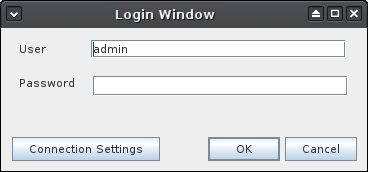
\includegraphics[width=0.5\linewidth]{img/auth_window.png}
		\caption{Authentication window}
		\label{fig:auth_window}
	\end{figure}
	The default connection settings should be enough if the server is running on the same computer the client is. If that's not the case, open the Connection Settings window (figure~\ref{fig:connection_settings}).
	\begin{figure}[h!]
		\centering
		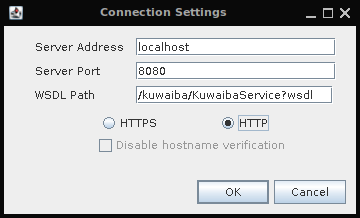
\includegraphics[width=0.5\linewidth]{img/connection_settings.png}
		\caption{Connection Settings window}
		\label{fig:connection_settings}
	\end{figure}
	\begin{itemize}
		\item \textbf{Server Address} Refers to the server IP address or canonical name.
		\item \textbf{Server Port} is the port Glassfish (the application server) is listening to.
		\item \textbf{WSDL Path} is the path within the application server the web service interface definition can be found. Usually this value should remain unchanged.
		\item Protocol is the transport protocol to be used. By default is HTTP, but is highly advisable to request your administrator to setup a secure connection, otherwise your credentials will be transmitted in plain text over the network. 
	\end{itemize}
	Except for the password, the last successful settings will be saved upon clicking OK.
	\begin{framed} {\large \textbf{Important}} \\
		If you are unsure if the server is reachable from your location, open a browser and type the address: \textbf{http://[server\_address]:[server\_port]/[wsdl\_location]}\\
		
		You should see a large XML document.
	\end{framed}
	\begin{framed} {\large \textbf{Troubleshooting}}
		\begin{itemize}
			\item For a \textbf{\textcolor{red}{Can't contact backend}} error, check the Administrator's Manual Troubleshooting section.
			\item If you get a \textbf{\textcolor{red}{Connection refused}} error, check the connection settings and verify that the server is reachable and there isn't a firewall blocking the traffic to it.
		\end{itemize}
	\end{framed} 
	Once you are logged in, you will see only the dashboard page and a toolbar (figure~\ref{fig:main_toolbar}).\\
	\begin{figure}[h!]
		\centering
		
\includegraphics[width=0.7\linewidth]{img/main_toolbar.png}
		\caption{Main toolbar}
		\label{fig:main_toolbar}
	\end{figure}
	
	The toolbar contains the most frequently used tools. Here is an overview of what cab you do with them:
	\begin{table}[h!]
		\centering
		\begin{tabular}{cl}
			
\includegraphics[width=0.5cm]{img/icon_query_manager.png} & Search objects with the Query Manager\\
			\midrule
			
\includegraphics[width=0.5cm]{img/icon_refresh_component.png} & Refresh the current view\\
			\midrule
			
\includegraphics[width=0.5cm]{img/icon_refresh_cache.png} & Refresh local cache\\
			\midrule
			
\includegraphics[width=0.5cm]{img/icon_object_view.png} & Physical/Rack View of an object\\
			\midrule
			
\includegraphics[width=0.5cm]{img/icon_task_manager.png} & Create automation tasks (beta version)\\
			\midrule
			
\includegraphics[width=0.5cm]{img/icon_audit_trail.png} & See the changes made to inventory and application objects\\
			\midrule
			
\includegraphics[width=0.5cm]{img/icon_user_manager.png} & Manage users and groups\\
			\midrule
			
\includegraphics[width=0.5cm]{img/icon_data_model_manager.png} & Change the data model\\
			\midrule
			
\includegraphics[width=0.5cm]{img/icon_containment_manager.png} & Manage how objects can be created inside others\\
			\midrule
			
\includegraphics[width=0.5cm]{img/icon_list_type_manager.png} & Create new list types\\
			\midrule
			
\includegraphics[width=0.5cm]{img/icon_topology_designer.png} & Freely design network topologies\\
			\midrule
			
\includegraphics[width=0.5cm]{img/icon_navigation_tree.png} & Main tree used to explore physical assets\\
			\midrule
			
\includegraphics[width=0.5cm]{img/icon_pools_manager.png} & Create and manage objects that don't fit in the navigation tree\\
			\midrule
			
\includegraphics[width=0.5cm]{img/icon_service_manager.png} & Manage client, services and resources associated to them\\
		\end{tabular}	
		\caption{Toolbar items}
		\label{tab:toolbar_icons}
	\end{table}
	
	\newpage
	\section{Data Model Manager} \label{sec:data_model_manager}
		One of the key features of Kuwaiba is that it is completely object-oriented\footnote{Object-oriented Programming https://en.wikipedia.org/wiki/Object-oriented\_programming}. It means that every business (Router, City, Port) and application (users, types) element is represented by an \textbf{Object} in the application and these objects are in turn product of an reality abstraction called \textbf{Class}. Likewise, every attribute is a \textbf{Field} in a class. The set of classes, attributes and relationships between them is called data model. There's a default data model, but you can customize it depending on your needs by adding, removing and modifying classes. To achieve this, use the Data Model Manager module (figure~\ref{fig:data_model_manager}).
		\begin{figure}[h!]
			\centering
			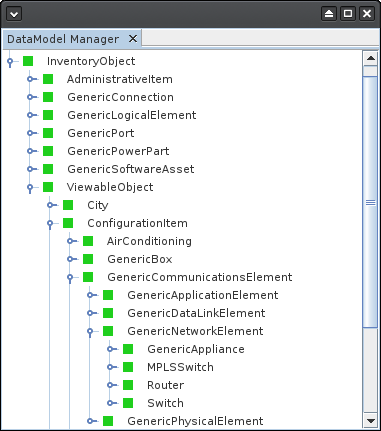
\includegraphics[width=0.4\linewidth]{img/data_model_manager.png}
			\caption{Part of the data model tree}
			\label{fig:data_model_manager}
		\end{figure}
		The data model is represented as a tree because it's a hierarchical structure. Technically, it's a class hierarchy\footnote{Class Hierarchy https://en.wikipedia.org/wiki/Class\_hierarchy}. The top of the hierarchy (\textbf{InventoryObject}) is the most general type of element in the data model and its subclasses represent all the possible elements that will be treated as inventory assets. As you dig deeper into the tree, the classes become more and more specialized and each level inherits the attributes of the parent classes. This kind of structure has two purposes: First, it helps you to organize your classes based on what characteristics they have in common. Secondly, as you will see later in this manual, you can apply operations over top level classes, and they will be propagated to all subclasses. Another root of the data model tree is \textbf{GenericObjectList}, and its subclasses are all possible list types (see more details on the subject in the chapter \textbf{\nameref{sec:list_type_manager}}).\newline
		
		\begin{framed} {\large \textbf{Important}} \\
				The \textbf{Properties} window allows you to modify the attributes of a selected object in a tree, list or view. If not already open, it's available from the Windows $\rightarrow$ Properties menu.
		\end{framed}
		The properties of a class can be edited by using the \textbf{Properties} window, selecting the class from the tree (see figure~\ref{fig:properties_class_node}). 
		\begin{figure}[h!]
			\centering
			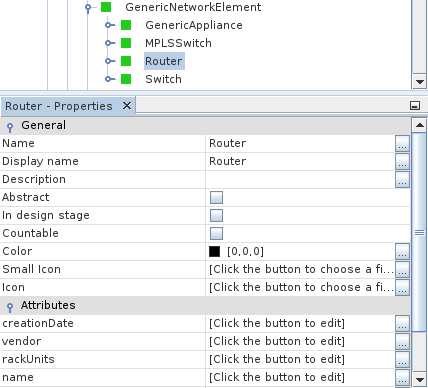
\includegraphics[width=0.5\linewidth]{img/properties_class_node.png}
			\caption{Properties of class \textbf{Router}}
			\label{fig:properties_class_node}
		\end{figure}
		The  property  sheet  is  divided  in  two  sections: 
		\begin{itemize}
			\item \textbf{General:} Contains the intrinsic properties  of  the class: \textbf{name} (can contain only letters and numbers with no special characters  or  blank  spaces). The  \textbf{display name} of the class, that's how the  will be displayed everywhere else (useful  for  internationalization  purposes, for example) and can contain any kind of UTF-8 character. A \textbf{description} (useful  to  document  the  data  model). If  the class is \textbf{abstract} (abstract classes  cannot  be  instantiated, they're only used to give consistency to the  data  model). The attribute \textbf{countable} is not used currently, but it should be used to mark classes whose instances can have graphical representations, but  they're  not really  part  of  the  inventory,  such  as  \textbf{Slots}. \textbf{In Design Stage} is just a way to mark a class as part of an ongoing data model intervention, and thus, classes with that attribute set to true can not be instantiated. \textbf{Color} is the color of the default square icon used to display the object in a tree or view. This icon will be used as long as the \textbf{Small Icon} attribute is null. \textbf{Small Icon} is the icon that will be used in trees and its size can't exceed 16x16 pixels. \textbf{Icon} is the icon used in views, and has a maximum size of 32x32 pixels.
			\begin{framed} {\large \textbf{Important}}
				\begin{itemize}
					\item All user-created classes are set In Design Stage = \textbf{\textcolor{green}{true}} by default. You won't be able to create objects of these classes until you set it to \textbf{\textcolor{blue}{false}}.
					\item As a convention, all abstract classes have the prefix \textbf{Generic}. Note that a few core classes (like \textbf{InventoryObject} or \textbf{\textcolor{green}{true}}) are abstract are the exception to this rule. You, however, should try to follow this convention as much as possible.
				\end{itemize}
			\end{framed}
			\item The second section  contains the class fields (attributes). In the  figure\ref{fig:properties_class_node}, class Router  has six attributes: name, state, conditions, vendor, serialNumber and creationDate. Click the button next to the attribute name to customize it (see figure~\ref{fig:class_attribute_details}).
			\begin{figure}[h!]
				\centering
				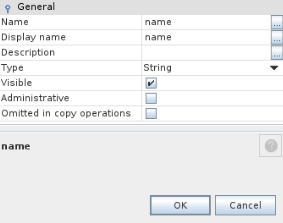
\includegraphics[width=0.4\linewidth]{img/class_attribute_details.png}
				\caption{Properties of attribute \textbf{name} in class \textbf{Router}}
				\label{fig:class_attribute_details}
			\end{figure}
		\end{itemize}
		In this window, you can modify the attribute's name, display name, description, type  (the drop-down list will show you primitive types -String, Integer, Float, Long, etc- and all available non-abstract list types). When you change an attribute's type, all existing instances will be	modified to reflect the change, which means that the values of the modified attribute will be converted to the new type if possible (say, from Integers to Strings). If the conversion is not possible, the new value will be set to null. You  can  also  manage  the  attribute  visibility. Attributes marked as “Administrative” will be shown in a separate tab in the object's property sheet. Sometimes, there are  attributes that are used only for administrative purposes and might confuse the end user if mixed with the regular attributes. Finally, you can choose what attributes shouldn't be transferred from one object to another in a copy operation.
		
		\begin{framed} {\large \textbf{Important}}
			\begin{itemize}
				\item You may lose information when changing an attribute's type. make sure the conversion to the new type is possible before you do it.
				\item Although there's a Cancel button at the bottom of the window, it does not	really work. When you perform a change, it's saved immediately.
			\end{itemize}
		\end{framed}
		You can also create and delete classes and attributes by right-clicking a class node (see figure~\ref{fig:class_node_menu})
		\begin{figure}[h!]
			\centering
			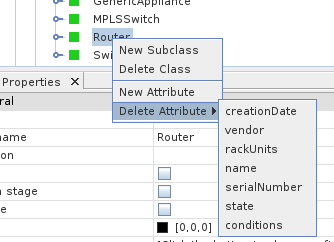
\includegraphics[width=0.4\linewidth]{img/class_node_menu.png}
			\caption{Class \textbf{Router} context menu}
			\label{fig:class_node_menu}
		\end{figure}
		New subclasses inherit the parent class attributes. Classes with instances or subclasses can not be deleted (this is  a  feature to avoid unintended loss of  data). Also, attribute \textbf{name} can not be deleted.
		\begin{framed} {\large \textbf{Important}}
			It's highly recommended \textbf{\textcolor{red}{NOT}} to rename abstract core classes, as some of them are used internally to support many features and renaming them may turn the system unstable.
		\end{framed}
		
	\newpage
	\section{Containment Manager} \label{sec:containment_manager}
	Another key concept in Kuwaiba is containment. It consists of the ability to define what kind of objects can be created within others. For example, a \textbf{Country} can be inside a \textbf{Continent}, but can't be inside a \textbf{Rack}. A \textbf{Port} is usually within a \textbf{Board}, and not inside a \textbf{City}. These business rules can be defined using the Containment Manager.
	
	\begin{figure}[h!]
		\centering
		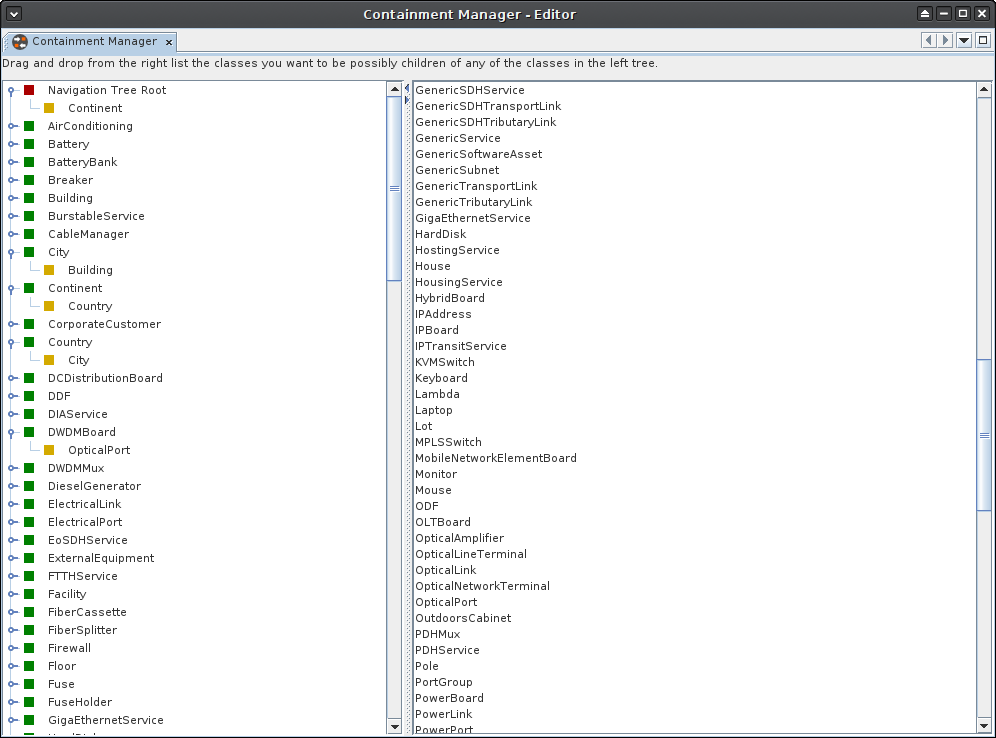
\includegraphics[width=0.7\linewidth]{img/containment_manager.png}
		\caption{Containment Manager main window. Zoom in the image to see the details}
		\label{fig:containment_manager}
	\end{figure}
	The main window is divided in two panels (see figure~\ref{fig:containment_manager}, zoom in the image to see the details). The one on the left is a tree that holds all the classes plus the \textbf{Navigation Tree Root}. The children of the left-side tree node are the possible classes that can be contained. In the figure~\ref{fig:containment_manager} there are five nodes expanded: \textbf{City}, that has one node inside: \textbf{Building}. That means that below a given city, you will only be able to add \textbf{Building} objects. Likewise, inside a \textbf{Continent} you can only create instances of \textbf{Country}, and inside those instances, only objects of class \textbf{City}. Under the root of the Navigation Tree, only instances of \textbf{Continent} are to be created. Finally, only \textbf{OpticalPorts} are supported under \textbf{DWDMBoards}. If for your operation Continents are not relevant, or if your routers do not have boards, but only ports, simplify the hierarchy as much as you want to meet your needs. To remove a possible children class, just right-click on it and select “Remove”, and instances from that class will no longer be available to be added under the parent class, though the objects created already will remain linked to the respective parent objects.
	\begin{framed} {\large \textbf{Important}}
		\begin{itemize}
			\item To avoid adding one by one many classes to a parent, you can use the flexibility of the data model as a hierarchical structure. For example, a \textbf{Rack} may contain within many types of equipment (routers, DDFs, switches, battery banks, etc). Instead of adding one by one each of these classes, you can add a common super class and all of them will be added automatically. For this example a common super class for most of those classes could be \textbf{GenericCommunicationsElement}.
			\item To search for a particular class, just select any node in the desired side of the panel and type the first letters of the class name. If there are many occurrences of the term, jump from one to another using the F3 key.
			\item The changes are applied immediately, however, if you happen to not see them reflected, press the Refresh Cache button 
\includegraphics[width=0.5cm]{img/icon_refresh_cache.png} in the main toolbar (see table~\ref{tab:toolbar_icons}).
		\end{itemize}
	\end{framed}
	\newpage
	
	\newpage
	\section{Navigation Tree} \label{sec:navigation_tree}
	This module presents in a tree fashion the physical objects of your inventory organized according to the containment hierarchy defined with the tool described in the previous chapter (see \textbf{\nameref{sec:containment_manager}}).
	\begin{figure}[h!]
		\centering
		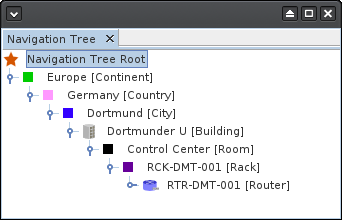
\includegraphics[width=0.4\linewidth]{img/navigation_tree.png}
		\caption{Navigation tree showing objects with default and user-defined icons}
		\label{fig:navigation_tree}
	\end{figure}
	Just like the \nameref{sec:data_model_manager}, the Properties window will display the attributes of the object selected in the Navigation Tree. These attributes match the visible attributes defined in the \textbf{\nameref{sec:containment_manager}}.
	\begin{figure}[h!]
		\centering
		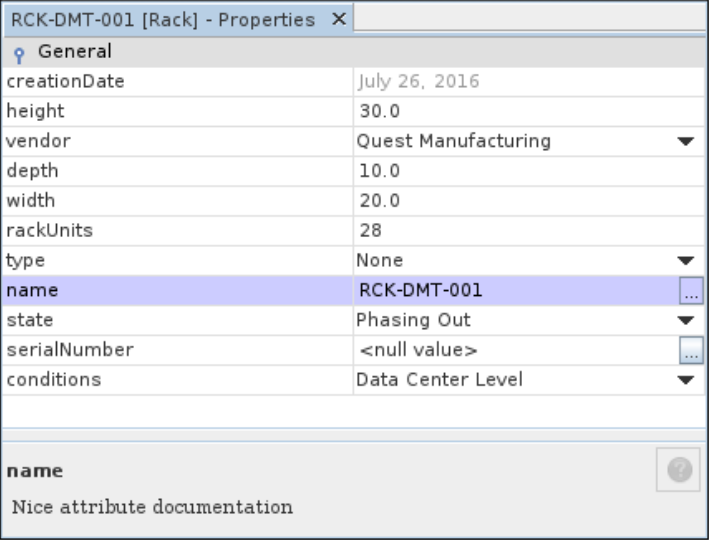
\includegraphics[width=0.5\linewidth]{img/navigation_tree_properties.png}
		\caption{Properties of a selected \textbf{Rack} object}
		\label{fig:navigation_tree_properties}
	\end{figure}
	Every change is automatically committed to the database once you hit the Enter key. When editing dates, you need to select another attribute to commit the changes instead of pressing Enter. In the \textbf{\nameref{sec:containment_manager}} you can also configure what labels will be displayed instead of the actual names of the attributes and the help string in the lowest part of the window.\newline
	
	Every node has a set of actions, some will be active for all objects, some depend on the type of element that is selected. In the figure~\ref{fig:navigation_tree_context_menu} you can see the actions enabled for a \textbf{Rack} object. \\
	\begin{figure}[h!]
		\centering
		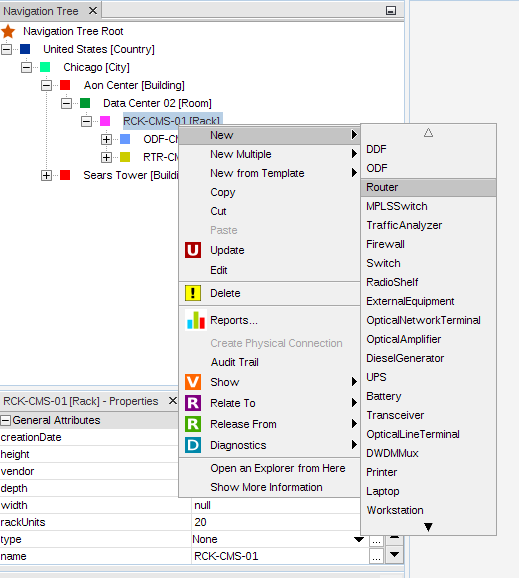
\includegraphics[width=0.5\linewidth]{img/navigation_tree_context_menu.png}
		\caption{Properties of a selected \textbf{Rack} object}
		\label{fig:navigation_tree_context_menu}
	\end{figure}
	\begin{itemize}
		\item \textbf{New Object:} The list of object types that can be contained for the selected element type according to the configured Containment Hierarchy. In this case, a \textbf{Rack} can only contain \textbf{Routers}.
		\item \textbf{Copy:} A plain copy operation.
		\item \textbf{Paste:} A plain paste operation. You can only paste objects where it is allowed according to the configured Containment Hierarchy.
		\item \textbf{Update:} Update the node information. Useful when a changed has made to the object from a external source (e.g. another user) or if you create a new list type affecting one of the attributes of the selected element. In this case, if you, for example, create an instance of \textbf{EquipmentVendor} (this will add a new entry to the \textbf{vendor} attribute list)
		\item \textbf{Delete:} Deletes the object. Tis will fail if the object has an incoming relationship, for example, a \textbf{Port} connected to a cable.
		\item \textbf{Reports:} The reports associate with this class. In this case, \textbf{Rack} has a report called \textbf{Rack Usage}. If no reports are associated, the option will appear grayed out.
		\item \textbf{Relate to service:} All inventory objects can be associated to an existing service. See more details in the chapter \nameref{sec:service_manager}.
		\item \textbf{Release from Service:} Removes the association between an object(resource) and a service. If the object is not related to any service, this option will appear grayed out.
		\item \textbf{Audit Trail:} This will display all the audit trail entries for the selected object, that is, all the changes made to the it.
		\item \textbf{Open an Explorer from this Node:} Opens a navigation tree whose root node will be the selected object. Useful when you want to explore an object with a many containment levels below.
		\item \textbf{Show Object Id:} Shows the database id of the selected object. Useful for troubleshooting purposes. It will also show the object's complete containment structure.
			\begin{figure}[h!]
				\centering
				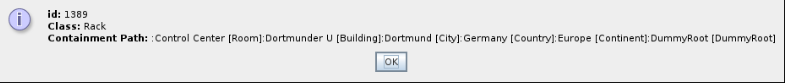
\includegraphics[width=\linewidth]{img/action_show_object_id.png}
				\caption{Object id action on the selected \textbf{Rack} object}
				\label{fig:action_show_object_id}
			\end{figure}
	\end{itemize}
	\begin{framed} {\large \textbf{Important}}
		\begin{itemize}
			\item Remember that you can always open the Properties window by selecting the main menu option Windows $\rightarrow$ Properties.
			\item You can change the name of an object in-line by pressing F2 on a selected node.
		\end{itemize}
	\end{framed}
	\subsection{Relationship and Special Children Explorer} \label{sec:extra_explorers}
	Apart from the main navigation tree, there are also two explorers that are very useful to navigate through domain-specific models. Both explorers are located in the Tools $\rightarrow$ Navigation menu.
	\begin{itemize}
		\item \textbf{Relationship Explorer:} Allows to see the special relationships of the selected object. When an object makes part of a domain-specific model (SDH, Physical Connections, MPLS, Software Licensing, etc) there are special bounds to other objects called \textbf{relationships} they have names documented on model-basis, and they can be seen using this explorer. In the figure~\ref{fig:navigation_tree_relationship_explorer}, it is depicted an \textbf{OpticalPort} with two relationships, one called \textbf{endpointA} used in the Physical Connections model and it indicates that this port is the endpoint to a physical connection, probably a fiber optic. It also has a relationship called \textbf{uses}, which makes part of the Service management model. It indicates that the service called PDH Service-01 uses that port as a resource.
			\begin{figure}[h!]
				\centering
				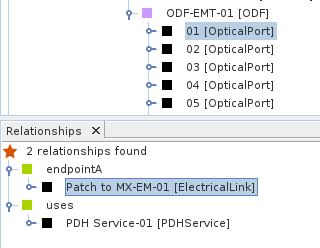
\includegraphics[width=0.4\linewidth]{img/navigation_tree_relationship_explorer.png}
				\caption{Special relationships of the selected \textbf{OpticalPort} object}
				\label{fig:navigation_tree_relationship_explorer}
			\end{figure}
		\item \textbf{Special Children Explorer:} The special children are children as in the containment hierarchy concept, but used in domain-specific models, which gives them particular behavior depending on the situation (that is, they can't be handled as simple objects in the navigation tree, because, for example, deleting them may require to perform other tasks but just removing the object from the database as they make part of a complex workflow). This is the case of the cables inside a conduit connecting two buildings. You can find more details about this scenario in the chapter \textbf{\nameref{sec:physical_connections}}.
			\begin{figure}[h!]
				\centering
				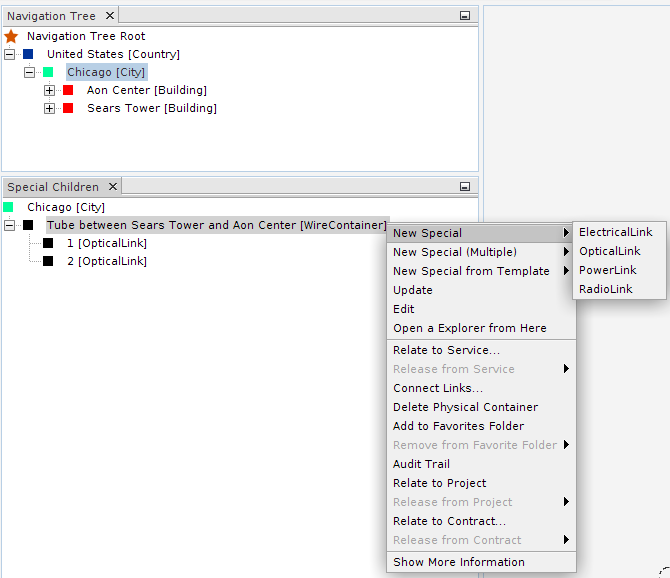
\includegraphics[width=0.3\linewidth]{img/navigation_tree_special_children_explorer.png}
				\caption{Fibers inside a container between two buildings}
				\label{fig:navigation_tree_special_children_explorer}
			\end{figure}
	\end{itemize}
	
	\newpage
	\section{List Type Manager} \label{sec:list_type_manager}
	Most of the attributes are primitive types (String, Integer, Booleans, etc), however, there are some more complex that point to another object in the database. This is the case of attributes such as \textit{vendor}, which points to an object holding the information about the vendor of that equipment (support lines, account manager, etc) or \textit{state}, that refers to the current operational state of the equipment (Working, Not Working, Stored, etc) and the state itself is an object, because it may hold information about what's the next allowed states, for example. Many objects in the database will have the same \textit{vendor}, and many other will have the same \textit{state}. In short, list types are those kind of attributes that point to an element in a limited set of objects. In terms of relational databases, you can see it as a many-to-one kind of relationships. To manage the existing list types and its instances, use the \textbf{\nameref{sec:data_model_manager}} and the \textbf{\nameref{sec:list_type_manager}}. \newline
	
	To add new list types, add a subclass under GenericObjectList directly or any of its utility subclasses. List types are like any other class, you can customize them as needed.
	\begin{figure}[h!]
		\centering
		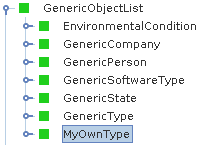
\includegraphics[width=0.3\linewidth]{img/list_type_own_type.png}
		\caption{Custom list type}
		\label{fig:list_type_own_type}
	\end{figure}
	 To create list type items, use the button 
\includegraphics[width=0.5cm]{img/icon_list_type_manager.png} or the menu option Tools $\rightarrow$ List Type Manager. This module consists of a simple navigation tree similar to the one seen in the past chapter.
	 \begin{figure}[h!]
	 	\centering
	 	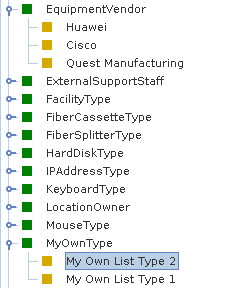
\includegraphics[width=0.3\linewidth]{img/list_type_list_type_items.png}
	 	\caption{Custom list type items}
	 	\label{fig:list_type_list_type_items}
	 \end{figure}
	 
	 By right-clicking and choosing \textit{New} on a selected list type, you can create new items. The details for every item can be edited using the standard Properties Window as seen in the past chapter. 
	 \newpage
	 \begin{framed} {\large \textbf{Important}}\\
	 	If the changes are not immediately reflected when editing an object, use the Refresh Cache button  
\includegraphics[width=0.5cm]{img/icon_refresh_cache.png} and update the object (Right-click the object node and select the option \textit{Update}).
	 \end{framed}
	 
	 In the figure~\ref{fig:list_type_applied_types} you can see the properties of an object of class \textbf{Router} modified to have an attribute called \textit{myOwnAttribute} of type \textbf{MyOwnListType}.\newline
	 \begin{figure}[h!]
	 	\centering
	 	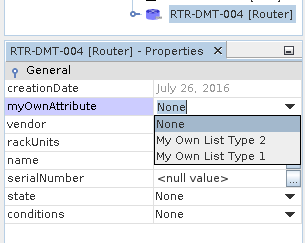
\includegraphics[width=0.4\linewidth]{img/list_type_applied_types.png}
	 	\caption{Object of class \textbf{Router} with a custom listy type attribute}
	 	\label{fig:list_type_applied_types}
	 \end{figure}
	 
	\newpage
	\section{Default and Rack Views}
	\subsection{Physical View} \label{sec:default_view}
		A view is a graphical representation of an object. There are many types of views, because an object has different perspectives, for example, a service object may have a view showing all the resources associated to it, a second view showing how all those resources are connected and a third showing statistics about such service. All instances (objects) of subclasses of \textbf{ViewableObject} have a Physical View that displays the direct children of the selected node. Most objects, except logical and administrative assets and a few physical ones such as slots and ports are subclasses of \textbf{ViewableObject}. To access this view, open the Physical View window (see \nameref{tab:toolbar_icons}) and select a node in the navigation tree.
		\begin{figure}[h!]
			\centering
			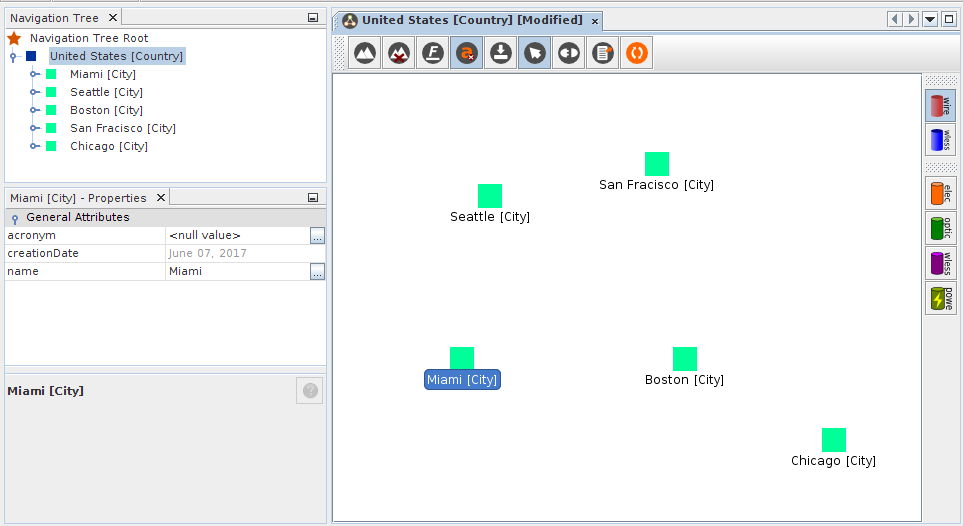
\includegraphics[width=0.9\linewidth]{img/default_view.png}
			\caption{Physical View of the selected \textbf{Country} object}
			\label{fig:default_view}
		\end{figure}
		
		In the Physical View, you can move and connect the nodes, add a background and export the view. It is particularly useful at Room and City levels, because it will allow you to see how the children elements are located geographically (e.g. buildings) or in an enclosed space (racks in a data center as seen in figure~\ref{fig:room_plan}).	
		\begin{figure}[h!]
			\centering
			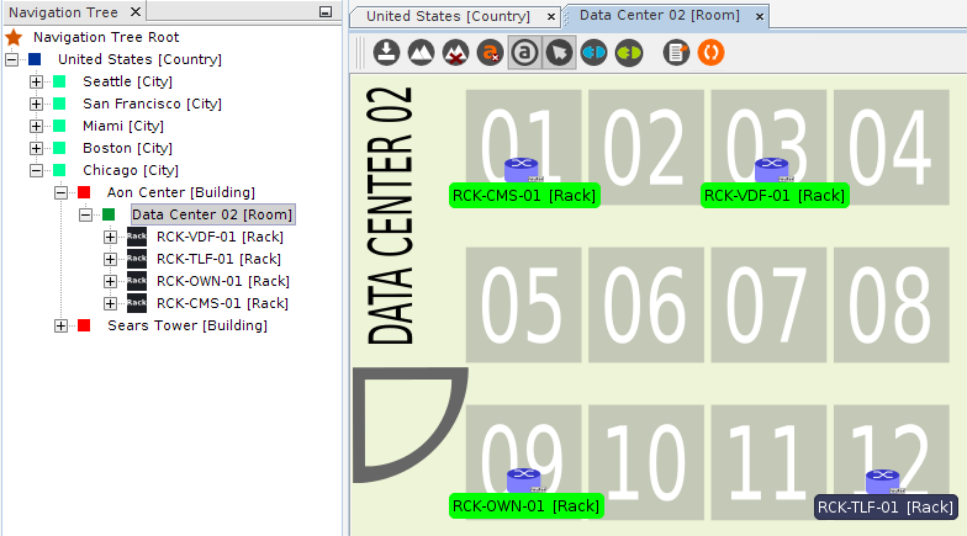
\includegraphics[width=0.7\linewidth]{img/room_plan.png}
			\caption{Physical View of the selected \textbf{Room} object}
			\label{fig:room_plan}
		\end{figure}
		
		The figure~\ref{fig:default_view_toolbar} shows all general purpose tools available in this window.
		\begin{figure}[h!]
			\centering
			
\includegraphics[width=0.6\linewidth]{img/default_view_toolbar.png}
			\caption{Physical View toolbar}
			\label{fig:default_view_toolbar}
		\end{figure}
		
		\begin{table}[h!]
			\centering
			\begin{tabular}[h!]{lp{10cm}}
				
\includegraphics[width=0.5cm]{img/icon_add_background.png} & Add background\\
				\midrule
				
\includegraphics[width=0.5cm]{img/icon_remove_background.png} & Remove background\\
				\midrule
				
\includegraphics[width=0.5cm]{img/icon_format_text.png} & Format text\\
				\midrule
				
\includegraphics[width=0.5cm]{img/icon_add_background.png} & Add background\\
				\midrule
				
\includegraphics[width=0.5cm]{img/icon_toggle_labels.png} & Hide/show the labels under the nodes\\
				\midrule
				
\includegraphics[width=0.5cm]{img/icon_save.png} & Save view\\
				\midrule
				
\includegraphics[width=0.5cm]{img/icon_add_background.png} & Add background\\
				\midrule
				
\includegraphics[width=0.5cm]{img/icon_select_tool.png} & Select/Move tool (selected by default)\\
				\midrule
				
\includegraphics[width=0.5cm]{img/icon_connect_tool.png} & Connect tool (See \textbf{\nameref{sec:physical_connections}} for more details on how to use it)\\
				\midrule
				
\includegraphics[width=0.5cm]{img/icon_export.png} & Export to image file\\
				\midrule
				
\includegraphics[width=0.5cm]{img/icon_refresh_view.png} & Refresh view\\
				\midrule
				\includegraphics[width=0.5cm]{img/icon_view_type.png} & View type. Currently, only the Physical (default) and Rack view are available (see \textbf{\nameref{sec:rack_view}} for more details on the latter)\\
			\end{tabular}
		\end{table}
		
		\subsection{Rack View} \label{sec:rack_view}
		This view works only with objects of class \textbf{Rack} or its subclasses. It shows how the elements contained within the selected object are organized, based on their positions and number of rack units used. 
		\begin{figure}[h!]
			\centering
			\includegraphics[width=0.2\linewidth]{img/rack_view_combobox.png}
			\caption{How to find the rack view in the toolbar}
			\label{fig:rack_view_combobox}
		\end{figure}
		
		For this view to be correctly built, two conditions must be met:
		\begin{itemize}
			\item The rack must have its \textbf{rackUnits} attribute set to a valid integer value. This attribute stores the total number rack units supported by the rack. Typical values are 20, 28, 34, 40 or 45.
			\begin{figure}[h!]
				\centering
				\includegraphics[width=0.6\linewidth]{img/error_rack_view_not_rackunits.png}
				\caption{Error displayed when the rack does not have a valid value of rack units}
				\label{fig:error_rack_view_not_rackunits}
			\end{figure}
			\item The attributes \textbf{rackUnits} and \textbf{position} must exist and set to valid values in the elements contained inside the rack. \textbf{rackUnits} in this case, makes reference to the number of rack units occupied by the contained element, while \textbf{position} is the start position of the contained element, 1-based, numbered from top to bottom. Your equipment vendor usually provides this value.
			\begin{figure}[h!]
				\centering
				\includegraphics[width=0.4\linewidth]{img/rack_view_attributes_contained_element.png}
				\caption{Attributes correctly set in a DDF contained inside a rack}
				\label{fig:rack_view_attributes_contained_element}
			\end{figure}
		\end{itemize}
		\begin{framed} {\large \textbf{Important}}
			\begin{itemize}
				\item The attribute names (\textbf{rackUnits}, \textbf{position}) are case sensitive and must be integers.
				\item Some elements you want to create inside a rack \textbf{might not} have those attributes by default, so you will need to create them using the \nameref{sec:data_model_manager}.			
			\end{itemize}
		\end{framed}
		If all values are correct, the view should look like this:
		\begin{figure}[h!]
			\centering
			\includegraphics[width=0.9\linewidth]{img/rack_view_sample_view.png}
			\caption{Sample rack view}
			\label{fig:rack_view_sample_view}
		\end{figure}
		
	\newpage
	\section{Physical Connections} \label{sec:physical_connections}
		The Physical Connections toolkit is tightly integrated to the Physical View module. With Kuwaiba you can create physical layer connections using cables, fiber optics or radio links very easily, navigate through the connections and inspect the resources in use.\newline
		
		Before presenting the tools provided by the application, let's first clarify and introduce some concepts. This module deals solely with L1 topologies. It's only about cables, ports, etc. The data model provides four types of entities to represent physical layer elements:
		\begin{itemize}
			\item \textbf{Connections:} These are all point-to-point physical links. In the current data model, there are three	types of connections: \textbf{ElectricalLink} (for electrical connections like coaxial, twisted
			pairs and the like), \textbf{OpticalLink} (for fiber optics) and \textbf{RadioLink} (for radio links -Microwave links, mostly-).
			\item \textbf{Containers:} All objects that can be used to contain, wrap and protect connections (understanding \textit{Connection} as defined above). There are two types of containers: \textbf{WireContainer} (used to contain all kind of cables -wires and fibers-, like pipes, conduits, ditches, etc) and \textbf{WirelessContainer} (used to contain radio channels or carriers).
			\item \textbf{Nodes:} These objects are endpoints to \textit{Containers}. In the default data model you will find classes like: \textbf{Tower}, \textbf{Warehouse}, \textbf{Facility}, \textbf{Shelter}, \textbf{Building}, \textbf{Floor} and \textbf{Room}, but in general, any subclass of \textbf{GenericPhysicalNode} can be a so called \textit{Node}.
			\textbf{Endpoints:} These objects are endpoints to \textit{Connections}. In practice, they're always some kind of \textbf{Port} (in the data model context, this means all subclasses of \textbf{GenericPort}).
		\end{itemize}
		In summary, you can only connect \textit{Nodes} using \textit{Containers} and \textit{Endpoints} using \textit{Connections}. To create new connections, select in the \textbf{\nameref{sec:navigation_tree}} an element and try to connected the desired children using the \nameref{sec:default_view}. For example, if you want to connect two buildings, select the city which is the parent for both. Likewise, if you want to connect a router to an ODF, you probably will have to select the room or the rack they are located. In short, select the nearest common parent between the two elements you want to connect.
		\begin{framed} {\large \textbf{Important}}\\
			You can also create power connections with this approach.
		\end{framed}
		\begin{table}[h!]
			\centering
			\begin{tabular}{lp{10cm}}
				\includegraphics[width=0.5cm]{img/icon_connect_tool.png} & Select the Connection tool \\
				\midrule
				\includegraphics[width=0.5cm]{img/icon_wire_container.png} & Create a wire container \\
				\midrule
				\includegraphics[width=0.5cm]{img/icon_wireless_container.png} & Create a wireless container \\
				\midrule
				\includegraphics[width=0.5cm]{img/icon_electrical_link.png} & Create an electrical link \\
				\midrule
				\includegraphics[width=0.5cm]{img/icon_optical_link.png} & Create an optical link \\
				\midrule
				\includegraphics[width=0.5cm]{img/icon_wireless_link.png} & Create a wireless link \\
			\end{tabular}
			\caption{Connection tools}
		\end{table}
		Let's put together all this concepts  with some examples. 
		\subsection{Example 1} \label{sec:physical_connections_example_1}
			In this example, we will create a direct connection between two routers in the same room, but in different racks using a CAT-5 patch as shown in the figure~\ref{fig:l1_example_1}.\newline
			\begin{figure}[h!]
				\centering
				\includegraphics[width=0.5\linewidth]{img/l1_example_1.png}
				\caption{Connection diagram for example 1}
				\label{fig:l1_example_1}
			\end{figure}
			
			Let's consider the layout in figure~\ref{fig:l1_example_1_layout}
			\begin{figure}[h!]
				\centering
				\includegraphics[width=0.3\linewidth]{img/l1_example_1_layout.png}
				\caption{Containment layout for example 1}
				\label{fig:l1_example_1_layout}
			\end{figure}
			\begin{enumerate}
				\item Select the nearest common parent in the navigation tree (in this case the \textbf{Room} called Control Center), and using the select tool, change the default position of the nodes
				\begin{figure}[h!]
					\centering
					\includegraphics[width=0.8\linewidth]{img/l1_example_1_initial_view.png}
					\caption{Racks in the room}
					\label{fig:l1_example_1_initial_view}
				\end{figure}
				\item Using the \textbf{\nameref{sec:list_type_manager}}, create a list type called \textit{CAT-5} under \textbf{ElectricalLinkType}. Following a similar procedure, you can create the different types of electrical connections depending on your network (POTS, coaxial, etc). We will use this later.
				\label{item:connection_type}
				\newpage
				\begin{figure}[h!]
					\centering
					\includegraphics[width=0.4\linewidth]{img/l1_example_1_electrical_link_type.png}
					\caption{Creating the link type}
					\label{fig:l1_example_1_electrical_link_type}
				\end{figure}
				\item Activating the connection tool, click on one node and hold, dragging the mouse until you reach the second node. Make sure you also select the type of connection you want to create, in this case, an \textbf{ElectricalLink} (a patch cable).
				\begin{figure}[h!]
					\centering
					\includegraphics[width=0.8\linewidth]{img/l1_example_1_new_connection.png}
					\caption{Creating the connection}
					\label{fig:l1_example_1_new_connection}
				\end{figure}
				\item This will open a wizard where you should select the endpoints of the connection (the end ports)
				\begin{figure}[h!]
					\centering
					\includegraphics[width=0.8\linewidth]{img/l1_example_1_endpoints.png}
					\caption{Connection wizard, step 1}
					\label{fig:l1_example_1_endpoints}
				\end{figure}
				\item In the next step of the wizard, you have to fill in the basic information about the connection: its name and type. Use the type we just created in step~\ref{item:connection_type}.
				\begin{figure}[h!]
					\centering
					\includegraphics[width=0.5\linewidth]{img/l1_example_1_basic_info.png}
					\caption{Connection wizard, step 2}
					\label{fig:l1_example_1_basic_info}
				\end{figure}
			\end{enumerate}
			
			And that's it. Double-clicking the connection will add a control point to it. You can add as many as you want, and control its route. The Properties window will get updated accordingly if you select the link or a node.
			\begin{figure}[h!]
				\centering
				\includegraphics[width=0.6\linewidth]{img/l1_example_1_final.png}
				\caption{Final result}
				\label{fig:l1_example_1_final}
			\end{figure}
			\begin{framed} {\large \textbf{Important}}\\
				Don't forget to save the view using the icon \includegraphics[width=0.5cm]{img/icon_save.png} in the toolbar, so your positioning changes are stored.
			\end{framed}
			
		\subsection{Example 2}	
			The second example is more complex. We will connect two buildings with a conduit that contains fibers. In each building there's a router and an ODF, one of the fiber pairs connecting the buildings, will be linking the two ODFs, and then, from the ODF, we'll patch our way the routers.
			\begin{figure}[h!]
				\centering
				\includegraphics[width=0.8\linewidth]{img/l1_example_2.png}
				\caption{Connection diagram for example 2}
				\label{fig:l1_example_2}
			\end{figure}
			\newpage
			We will use a similar containment layout for this example, just adding a couple ODFs.
			\begin{figure}[h!]
				\centering
				\includegraphics[width=0.4\linewidth]{img/l1_example_2_layout.png}
				\caption{Containment layout for example 2}
				\label{fig:l1_example_2_layout}
			\end{figure}
			
			\begin{enumerate}
					\item First, we must make the initial arrangements. In this case, we will use a Google maps image as background for the city (the nearest common parent) and locate the buildings. We also select the connection tool and the type of connection, which will be a \textbf{WireContainer} this time.  
					\begin{figure}[h!]
						\centering
						\includegraphics[width=\linewidth]{img/l1_example_2_initial_view.png}
						\caption{Buildings in the city}
						\label{fig:l1_example_2_initial_view}
					\end{figure}
					\newpage
					\item Since this time we are creating a \textbf{WireContainer}, the list type for it must be created under \textbf{WireContainerType}. Using the \nameref{sec:list_type_manager}, add this entry:
					\begin{figure}[h!]
						\centering
						\includegraphics[width=0.2\linewidth]{img/l1_example_1_wire_container_type.png}
						\caption{reating a connection type}
						\label{fig:l1_example_1_wire_container_type}
					\end{figure}
					\item Just like we did in the past example, let's start the connection wizard, but this time the endpoints will be the buildings instead of the ports (remember that we are creating a container here).
					\begin{figure}[h!]
						\centering
						\includegraphics[width=0.8\linewidth]{img/l1_example_2_endpoints.png}
						\caption{Connection wizard, step 1}
						\label{fig:l1_example_2_endpoints}
					\end{figure}			
					\item In the second step, we fill in the basic fields, but in addition to what we had seen already, it's also necessary to provide information about what's gonna be contained inside the \textbf{WireContainer} and how many of those elements are to be created. Since this example is about connecting fibers, we select \textbf{OpticalLink} in the field \textit{Children type} and 20 in \textit{Num of children} just for the sake of the example.
					\begin{figure}[h!]
						\centering
						\includegraphics[width=0.6\linewidth]{img/l1_example_2_basic_info.png}
						\caption{Connection wizard, step 2}
						\label{fig:l1_example_2_basic_info}
					\end{figure}
					\item Using the Select tool, modify the route of the connection. Now the container has been created successfully.
					\begin{figure}[h!]
						\centering
						\includegraphics[width=\linewidth]{img/l1_example_2_final.png}
						\caption{Final result}
						\label{fig:l1_example_2_final}
					\end{figure}
					\item Once the container has been created, we can now connect a pair of fibers to each side's ODF back port (note the naming used for the ODF ports in the figure~\ref{fig:l1_example_2_layout}). To start a wizard to perform this operation, right-click the container and select the option \textit{Connect links...}
					\begin{figure}[h!]
						\centering
						\includegraphics[width=0.3\linewidth]{img/l1_example_2_container_context_menu.png}
						\caption{Container's contextual menu}
						\label{fig:l1_example_2_container_context_menu}
					\end{figure}
					\item This open a window divided in three panels. The side panels let you choose what ports do you want to connect to the fibers in the container. In this example, we will connect the first pair to the ports labeled as \textit{Back} in the ODFs. You can select multiple ports and fibers and connect them at the same time (use the SHIFT key for multiple selection). Note that it's not necessary to connect both sides. Push the \textit{Connect} button on the lower part of the central panel to finish the procedure.
					\begin{figure}[h!]
						\centering
						\includegraphics[width=\linewidth]{img/l1_example_2_connect_links.png}
						\caption{Connecting links}
						\label{fig:l1_example_2_connect_links}
					\end{figure}
					\begin{framed} {\large \textbf{Important}}
						\begin{itemize}
							\item In optical connections, Rx and Tx ports are treated as a single port and a pair of fibers, are actually represented as a single \textbf{OpticalLink}.							
						\end{itemize}
					\end{framed}
					It's possible to explore the contents of a container and see to what fiber the ports are connected to using the explorers in the menu Tools $\rightarrow$ Navigation. In the figure~\ref{fig:l1_example_2_links_in_container} you will see the Special Children explorer when the container is selected in the view. In the figure~\ref{fig:l1_example_2_container_relationships}, the relationship explorer shows the connections of one of the ports in the ODF when selected in the \nameref{sec:navigation_tree}.
					\begin{figure}
						\centering
						\includegraphics[width=0.3\linewidth]{img/l1_example_2_links_in_container.png}
						\caption{Exploring the container's contents}
						\label{fig:l1_example_2_links_in_container}
					\end{figure}
					\begin{figure}
						\centering
						\includegraphics[width=0.4\linewidth]{img/l1_example_2_container_relationships.png}
						\caption{Exploring the container's relationships}
						\label{fig:l1_example_2_container_relationships}
					\end{figure}
					\item Now we will create an optical patch on each building between the routers and the 1-Front ports of their respective ODFs in a similar way we did in the \textbf{\nameref{sec:physical_connections_example_1}}.
					\begin{figure}[h!]
						\centering
						\includegraphics[width=0.5\linewidth]{img/l1_example_2_patch_a.png}\\
						\includegraphics[width=0.5\linewidth]{img/l1_example_2_patch_b.png}
						\caption{Optical patches between routers and ODFs}
						\label{fig:l1_example_2_patches}
					\end{figure}
					\begin{framed} {\large \textbf{Important}}\\
							Remember to use an \textbf{OpticalLink} \includegraphics[width=0.5cm]{img/icon_optical_link.png} instead of an \textbf{ElectricalLink} \includegraphics[width=0.5cm]{img/icon_electrical_link.png}.							
					\end{framed}
					\item There's still one last step: The ports 1-Front and 1-Back in each ODF are not yet bridged. To do this, we just have to right-click any of the two ports on each ODF and select the option \textit{Connect Mirror Port...}. A mirror port is basically a direct connection between two ports. A cable is a separate object in Kuwaiba, a mirror connection is not even an object, is just a relationship between a port an another with the same parent (that is, a sibling). You can see it as a backplane connection.
					\begin{figure}[h!]
						\centering
						\includegraphics[width=0.5\linewidth]{img/l1_example_2_mirror_connection_menu.png}
						\caption{Mirror connection menu}
						\label{fig:l1_example_2_mirror_connection_menu}
					\end{figure}
					\newpage
					This will open a window where you can select what port do you want to be mirror of the selected one. Since 1-Front ports only have one sibling (1-Back), that's the only option available.
					\begin{figure}[h!]
						\centering
						\includegraphics[width=0.5\linewidth]{img/l1_example_2_mirror_connection_details.png}
						\caption{Mirror connection details}
						\label{fig:l1_example_2_mirror_connection_details}
					\end{figure}
					
					Once the port is mirrored, you can see a new relationship in the relationship explorer when selecting any of the ODF ports in the \textbf{\nameref{sec:navigation_tree}}.
					\begin{figure}[h!]
						\centering
						\includegraphics[width=0.4\linewidth]{img/l1_example_2_mirror_connection_relationships.png}
						\caption{Mirror connection relationship}
						\label{fig:l1_example_2_mirror_connection_relationships}
					\end{figure}
					
					To release a mirror port, select the option from the context port's context menu.
					\begin{figure}[h!]
						\centering
						\includegraphics[width=0.3\linewidth]{img/l1_example_2_mirror_connection_release.png}
						\caption{Release mirror connection menu option}
						\label{fig:l1_example_2_mirror_connection_release}
					\end{figure}
			\end{enumerate}
			
			A nice feature in Kuwaiba is the ability to see the path of a physical connection as long as there's continuity. In our example, there is continuity between the port in the router A (RTR-DMT-003) and the port in the Router B (RTR-DMT-004), that is, there are no active elements in between. To see the trace, right-click on any of the ports involved in the connection and select the option \textit{Show physical path}.
			\begin{figure}[h!]
				\centering
				\includegraphics[width=0.3\linewidth]{img/l1_example_2_physical_path_menu.png}
				\caption{Physical path menu option}
				\label{fig:l1_example_2_physical_path_menu}
			\end{figure}
			The figure~\ref{fig:l1_example_2_physical_path_list} show the physical path between Router A's port and Router B's port. The port in red is where the trace begins.
			\begin{figure}[h!]
				\centering
				\includegraphics[width=0.4\linewidth]{img/l1_example_2_physical_path_list.png}
				\caption{Physical path details}
				\label{fig:l1_example_2_physical_path_list}
			\end{figure}
			
			And pressing the button \includegraphics[width=0.5cm]{img/icon_physical_path_graphical.png} you will get a graphical representation, easier to understand.
			\begin{figure}[h!]
				\centering
				\includegraphics[width=1.1\linewidth]{img/l1_example_2_physical_path_view.png}
				\caption{Physical path graphical representation}
				\label{fig:l1_example_2_physical_path_view}
			\end{figure}
			The Properties window will be updated as you select any of the blocks. This view can also be updated.
	\newpage
	\section{Audit Trail} \label{sec:audit_trail}
	Kuwaiba is capable of tracking the changes performed by the users in the database for audit purposes. These changes can be made to inventory objects (equipment, locations, etc) or application objects (pools, tasks, user properties). There are two types of events that are logged: \textbf{General events}, that is, those that are not related to any object in particular, like new logins or creation of application objects. \textbf{Object-related events}, like property changes or move operations.
	\begin{figure}[h!]
		\centering
		\includegraphics[width=\linewidth]{img/audit_trail_general_events.png}
		\caption{General events window}
		\label{fig:audit_trail_general_events}
	\end{figure}
	
	The figure~\ref{fig:audit_trail_general_events} shows the window displayed after pressing the \textbf{\nameref{sec:audit_trail}} button \includegraphics[width=0.5cm]{img/icon_audit_trail} (or selecting the menu option Tools $\rightarrow$ Audit Trail). It shows the general events, paginated and chronologically sorted from the oldest to the newest event.
	\begin{table}[h!]
		\centering
		\begin{tabular}{lp{10cm}}
			\includegraphics[width=0.5cm]{img/icon_export.png} & Export to CSV file \\
			\midrule
			\includegraphics[width=0.5cm]{img/icon_retrieve_all.png} & Retrieve all log entries (may take some time depending on the number of records) \\
			\midrule
			\includegraphics[width=0.5cm]{img/icon_previous_page.png} & Previous page \\
			\midrule
			\includegraphics[width=0.5cm]{img/icon_next_page.png} & Next page \\
		\end{tabular}
		\caption{Audit trail toolbar icons}
	\end{table}
	
	The object-related audit trail window is very similar, but contains only the events related to the selected node. To see the audit trail, select a node in a tree or view, right-click on it and select the \textit{Audit Trail} option.
		\begin{figure}[h!]
			\centering
			\includegraphics[width=0.5\linewidth]{img/audit_trail_menu_option.png}
			\caption{Audit trail menu option}
			\label{fig:audit_trail_menu_option}
		\end{figure}
		\newpage
		The result is not paginated, but can be exported to a CSV file.
		\begin{figure}[h!]
			\centering
			\includegraphics[width=\linewidth]{img/audit_trail_object_related_events.png}
			\caption{\textbf{Router} object audit trail}
			\label{fig:audit_trail_object_related_events}
		\end{figure}
	\newpage
	\section{Topology Designer} \label{sec:topology_designer}
		Use this module to make sketches of your network, but using the equipment already created in the inventory. Most people use applications like MS Power Point\texttrademark, MS Visio\texttrademark  or a CAD program for this, but here it is already integrated. Use the button \includegraphics[width=0.5cm]{img/icon_topology_designer.png} in the main toolbar to open the designer.
		\begin{table}[h!]
			\centering
			\begin{tabular}{lp{10cm}}
				\includegraphics[width=0.5cm]{img/icon_new_element.png} & New topology \\
				\midrule
				\includegraphics[width=0.5cm]{img/icon_open.png} & Open topology \\
				\midrule
				\includegraphics[width=0.5cm]{img/icon_save.png} & Save topology \\
				\midrule
				\includegraphics[width=0.5cm]{img/icon_delete.png} & Delete topology/Clear canvas \\
				\midrule
				\includegraphics[width=0.5cm]{img/icon_export.png} & Export topology to image file \\
				\midrule
				\includegraphics[width=0.5cm]{img/icon_select_tool.png} & Select tool \\
				\midrule
				\includegraphics[width=0.5cm]{img/icon_connect_tool.png} & Connect tool \\
				\midrule
				\includegraphics[width=0.5cm]{img/icon_cloud.png} & Insert cloud \\
				\midrule
				\includegraphics[width=0.5cm]{img/icon_frame.png} & Insert frame \\
				\midrule
				\includegraphics[width=0.5cm]{img/icon_add_background.png} & Add background \\
				\midrule
				\includegraphics[width=0.5cm]{img/icon_remove_background.png} & Remove background \\
			\end{tabular}
			\caption{Topology Designer toolbar icons}
			\label{tab:topology_designer_icons}
		\end{table}
		\begin{framed} {\large \textbf{Important}}\\
			The connections made using this module are not actual inventory objects (unlike those seen in the chapter \textbf{\nameref{sec:physical_connections}}), simply lines linking nodes.							
		\end{framed}
		
		For starters, drag objects from the \textbf{\nameref{sec:navigation_tree}} onto the canvas of the view. You can add equipment (routers, switches, multiplexers) or locations (buildings, outdoor cabinets, poles, etc). If you have previously set the \textit{icon} of the classes the object you have dragged are instance of, it will be used, otherwise, a colored squared will be used instead to represent the nodes. In the figure~\ref{fig:topology_designer_initial_view} there are two routers and an object of class \textbf{ExternalEquipment}. 
		\begin{figure}[h!]
			\centering
			\includegraphics[width=0.6\linewidth]{img/topology_designer_initial_view.png}
			\caption{Sample topology without connections}
			\label{fig:topology_designer_initial_view}
		\end{figure}
		
		You can add nodes that are not inventory objects, but that can help to decorate the topology. If you click the cloud button \includegraphics[width=0.5cm]{img/icon_cloud.png}, a cloud will be added to the topology. If the Selection tool is activated \includegraphics[width=0.5cm]{img/icon_select_tool.png}, drag the nodes to position them as needed. You can also add a frame by clicking the frame button \includegraphics[width=0.5cm]{img/icon_frame.png}. The name of the nodes can be changed by double-clicking them. The label of a frame can also be changed by double-clicking its border.
		\begin{figure}[h!]
			\centering
			\includegraphics[width=0.8\linewidth]{img/topology_designer_extra_nodes.png}
			\caption{Same topology, but adding a cloud and a frame}
			\label{fig:topology_designer_extra_nodes}
		\end{figure}
		
		To resize a frame, click on a corner and drag until you get the desired size. To create connections, select the Connection tool and link two nodes as you did in the \textbf{\nameref{sec:physical_connections}} chapter.
		\begin{figure}[h!]
			\centering
			\includegraphics[width=\linewidth]{img/topology_designer_connections.png}
			\caption{Topology with connections}
			\label{fig:topology_designer_connections}
		\end{figure}
		
		Don't forget to save the topology with pressing the Save button \includegraphics[width=0.5cm]{img/icon_save.png}. If saved, this topology can be loaded later using the Open button  \includegraphics[width=0.5cm]{img/icon_open.png}
		
	\newpage
	\section{Service Manager} \label{sec:service_manager}
	
	\newpage
	\section{Contract Manager} \label{sec:contract_manager}
		This small module allows you to organize your contracts in pools and keep track of the expiration dates and service providers. To open it, use the menu option Tools $\rightarrow$ Advanced $\rightarrow$ Contract Manager.
		\begin{figure}[h!]
			\centering
			\includegraphics[width=0.5\linewidth]{img/contract_manager_new_contract_pool.png}
			\caption{Creating a Contract Pool}
			\label{fig:contract_manager_new_contract_pool}
		\end{figure}
		
		The contracts are stored in pools, so first, you need to create your contract structure. Right click on the root node and select \textit{New Contract Pool}. Then, inside the pools create the contracts you want, and set their properties.
		\begin{figure}[h!]
			\centering
			\includegraphics[width=0.4\linewidth]{img/contract_manager_editing_properties.png}
			\caption{Editing a contract}
			\label{fig:contract_manager_editing_properties}
		\end{figure}		
		\begin{framed} {\large \textbf{Important}}\\
			If you are editing a date, so it can be set correctly, instead of just hitting the Enter key, change the focus to other attribute in the property sheet (that is, select another property with the mouse).							
		\end{framed}
		To create a service provider for the contracts, go to the \textbf{\nameref{sec:list_type_manager}} and create an entry under \textbf{ServiceProvider}.
		\begin{figure}[h!]
			\centering
			\includegraphics[width=0.2\linewidth]{img/contract_manager_service_providers.png}
			\caption{New service provider}
			\label{fig:contract_manager_service_providers}
		\end{figure}
		
		Any inventory object can be subject to a contract. You can associate an element to an existing contract, right click on it ans select the option \textit{Associate to contract...} and select the desired one as shown in the figure~\ref{fig:contract_manager_contract_list}.
		\begin{figure}[h!]
			\centering
			\includegraphics[width=0.4\linewidth]{img/contract_manager_associate_option.png}
			\caption{Associate to contract option}
			\label{fig:contract_manager_associate_option}
		\end{figure}		
		\newline
		\begin{figure}[h!]
			\centering
			\includegraphics[width=0.4\linewidth]{img/contract_manager_contract_list.png}
			\caption{Contract list}
			\label{fig:contract_manager_contract_list}
		\end{figure}
		
		The new elements associated to a contract are also available in the Contract Manager window.
		\begin{figure}[h!]
			\centering
			\includegraphics[width=0.4\linewidth]{img/contract_manager_elements.png}
			\caption{Elements associated to a contract}
			\label{fig:contract_manager_elements}
		\end{figure}
		
		This association can be undone either from the \textbf{\nameref{sec:navigation_tree}} or the \textbf{Contract Manager} using the node's context menu.
		\begin{figure}[h!]
			\centering
			\includegraphics[width=0.6\linewidth]{img/contract_manager_release_from_contract.png}
			\caption{Removing the association}
			\label{fig:contract_manager_release_from_contract}
		\end{figure}
		
	\newpage
	\section{Task Manager} \label{sec:task_manager}
		The Task Manager is the early release of a complete automation and notification module. At this stage, you can create tasks, edit a script that will be executed and execute this task either on demand or associated to a Dashboard widget that will be loaded at user login time. To open the Task Manager, select the menu option Tools $\rightarrow$ Task Manager or press the button \includegraphics[width=0.5cm]{img/icon_task_manager.png} in the main toolbar.
		\begin{figure}[h!]
			\centering
			\includegraphics[width=0.3\linewidth]{img/task_manager_create_task.png}
			\caption{Creating a new task}
			\label{fig:task_manager_create_task}
		\end{figure}
		Right-clicking the root node of the task tree will present a menu to create tasks. A task object has the following attributes
		\begin{table}[h!]
			\centering
			\begin{tabular}{lp{10cm}}
				\textbf{name} & The name of the task. \\
				\midrule
				\textbf{description} & The description of the task. \\
				\midrule
				\textbf{enabled} & Is this task enabled? \\
				\midrule
				\textbf{script} & The Groovy script to be executed by this task.\\
				\midrule
				\textbf{startTime} & The exact time and date this task shoud start its execution. Applicable only to tasks with \textit{executionType} set to Loop. 
				\textbf{Not used yet}. \\
				\midrule
				\textbf{everyXMinutes} & After the start time, every how many minutes should this task be executed? Applicable only to tasks with \textit{executionType} set to Loop. \textbf{Not used yet}.\\
				\textbf{executionType} & How should the task be executed.
					\begin{itemize}
						\item On Demand: Run only if the user executes it manually.
						\item User Login: Run upon subscribed users login.
						\item Loop: Run on a periodic basis, using the parameters described above.
						\item System Startup: Run when the system goes up.
					\end{itemize}
					Currently, only \textit{On Demand} and \textit{User Login} are used\\
				\midrule
				\textbf{email} & The email of the person or group that will receive the notification. Optional. \textbf{Not used yet}.\\
				\midrule
				\textbf{notificationType} & What type of notification should the subscribed users receive?
					\begin{itemize}
						\item No Notification: No notification.
						\item Client Managed: The client that executes the task decides how to notify.
						\item Email: Send an email to the address described above.
					\end{itemize}
					\textbf{Not used yet}.
			\end{tabular}
		\end{table}
		
		It is possible to subscribe users, so that they receive notifications with the result of the execution. Right-click on the task node, select the option \textit{Subscribe users...} and pick a user from the list.
		\begin{figure}[h!]
			\centering
			\includegraphics[width=0.3\linewidth]{img/task_manager_subscribe_users.png}
			\caption{Subscribing a user}
			\label{fig:task_manager_subscribe_users}
		\end{figure}
		
		It is out of the scope of this document to teach how to code scripts, however, in the directory \textbf{scripts} of the client installer, you will find some samples to guide you through. It's important to note, though, that most of the times, the scripts will require input parameters. This parameters can be easily added to the task so the user can fill them in before to run the task. To create parameters, right-click the task node and select the option \textit{Add Parameter...}
		\begin{figure}[h!]
			\centering
			\includegraphics[width=0.3\linewidth]{img/task_manager_add_parameter.png}
			\caption{Adding a parameter}
			\label{fig:task_manager_add_parameter}
		\end{figure}
		
		Once added, it will be immediately available in the property sheet, under the category \textit{Task Parameters}.
		\begin{figure}[h!]
			\centering
			\includegraphics[width=0.5\linewidth]{img/task_manager_property_sheet.png}
			\caption{Subscribing a user}
			\label{fig:task_manager_property_sheet}
		\end{figure}
		
		Tasks can also be executed on-demand. To do that, select the \textit{Execute Task} option from the task node's context menu.
		\begin{figure}[h!]
			\centering
			\includegraphics[width=1.1\linewidth]{img/task_manager_execute_task.png}
			\caption{Task execution}
			\label{fig:task_manager_execute_task}
		\end{figure}
		\begin{framed} {\large \textbf{Important}}\\
			The full set of methods available in a script can be found at \\ \tiny{http://kuwaiba.org/javadoc/persistence/org/kuwaiba/apis/persistence/interfaces/ApplicationEntityManager.html}
		\end{framed}
	\newpage
	\section{SDH Networks}
		This module allows to create end-to-end virtual circuits and all other logical entities required by the SDH protocol\footnote{SDH Graphical Overview http://www.cisco.com/c/en/us/support/docs/optical/synchronous-digital-hierarchy-sdh/28327-sdh-28327.html}. Let's introduce some concepts first. See figure~\ref{fig:sdh_module_description} for sample connection that illustrate the following terms.
		\begin{enumerate}
			\item \textbf{TransportLink:} A point-to-point logical connection that represents a single STMX. By default, the \textbf{TransportLinks} included in Kuwaiba are SMT1, STM4, STM16, STM64 and STM256.
			\item \textbf{ContainerLink:} It's a  logical connection that may or may not have multiple hops and connects ports within the boundaries of the transport network. A \textbf{ContainerLink} ends where at least one \textbf{TransporLink} ends, but in its path, the \textbf{ContainerLink} may have used many \textbf{TransportLinks}. In simple terms, a ContainerLink is an SDH virtual circuit. By default there are defined 5 types of ContainerLinks: VC12, VC3, VC4, VC4x4 and VC4x16. The latter two provide support for concatenation.
			\item \textbf{TributaryLink:} Objects of this types are not circuits themselves, they rather use actual virtual circuits (ContainerLinks) and end in the ports where the SDH service is delivered to the customer (usually tributary ports).
		\end{enumerate}
		In short, Transport and ContainerLinks provide the foundations for the hierarchy, while the TributaryLinks provide information about where the circuits are delivered (that is, what are the endpoints of the connections). Detailed information about the data model portion devoted to SDH, read the document \textit{SDH Model and Tools}.
		\newpage
		\begin{landscape}
			\begin{figure}
				\centering
				\includegraphics[width=\linewidth]{img/sdh_module_description.png}
				\caption{Sample multi-hop SDH circuit and its relationships with services, customers and physical resources}
				\label{fig:sdh_module_description}
			\end{figure}
		\end{landscape}
		\newpage
		To create an SDH topology, go to the menu option Tols $\rightarrow$ Advanced $\rightarrow$ SDH Networks. This will open an empty canvas similar to the \nameref{sec:topology_designer}.
		\begin{table}[h!]
			\centering
			\begin{tabular}{lp{10cm}}
				\includegraphics[width=0.5cm]{img/icon_new_element.png} & New topology \\
				\midrule
				\includegraphics[width=0.5cm]{img/icon_open.png} & Open topology \\
				\midrule
				\includegraphics[width=0.5cm]{img/icon_save.png} & Save topology \\
				\midrule
				\includegraphics[width=0.5cm]{img/icon_delete.png} & Delete topology/Clear canvas \\
				\midrule
				\includegraphics[width=0.5cm]{img/icon_export.png} & Export topology to image file \\
				\midrule
				\includegraphics[width=0.5cm]{img/icon_select_tool.png} & Select tool \\
				\midrule
				\includegraphics[width=0.5cm]{img/icon_connect_tool.png} & Connect tool \\
				\midrule
				\includegraphics[width=0.5cm]{img/sdh_module_transport_link.png} & Create a \textbf{TransportLink} \\
				\midrule
				\includegraphics[width=0.5cm]{img/sdh_module_container_link.png} & Create a \textbf{ContainerLink} \\
				\midrule
				\includegraphics[width=0.5cm]{img/sdh_module_tributary_link.png} & Create \textbf{TributaryLink} \\
			\end{tabular}
			\caption{SDH module toolbar icons}
			\label{tab:sdh_module_icons}
		\end{table}
		
		Drag and drop the equipment you need from the \nameref{sec:navigation_tree} and place them on the canvas.
		\begin{figure}[h!]
			\centering
			\includegraphics[width=\linewidth]{img/sdh_module_initial_view.png}
			\caption{Some routers and multiplexers in an SDH topology}
			\label{fig:sdh_module_initial_view}
		\end{figure}
		
		Let's consider this 4 equipment topology. What we are going to do, is to create a ring using STM-4 on one branch and SMT-1 on the other. We will create a VC12 between \textbf{SDH-87} and \textbf{Router 1}. Each equipment has the same board/port layout: Two boards, a tributary and an aggregate one, with two ports each.
		\begin{figure}[h!]
			\centering
			\includegraphics[width=0.4\linewidth]{img/sdh_module_layout.png}
			\caption{Port/board layout}
			\label{fig:sdh_module_layout}
		\end{figure}
		
		First, we have to create the most basic support, that is the TransportLinks (STMX). Use the Connect tool \includegraphics[width=0.5cm]{img/icon_connect_tool.png} and press the Create TransportLink button \includegraphics[width=0.5cm]{img/sdh_module_transport_link.png}. Then, just like the \nameref{sec:topology_designer} and the \nameref{sec:physical_connections}, drag a line from one equipment to the other. That will start a wizard.\newline
		
		To change the connection color, use the \nameref{sec:data_model_manager}. Select the class corresponding to the desired TransportLink and change the attribute \textit{color}.
		\begin{figure}[h!]
			\centering
			\includegraphics[width=0.6\linewidth]{img/sdh_module_transport_link_color.png}
			\caption{Changing the color for STM1 links}
			\label{fig:sdh_module_transport_link_color}
		\end{figure}
		
		The first step of the wizard will request for the basic information: name and type
		\begin{figure}[h!]
			\centering
			\includegraphics[width=\linewidth]{img/sdh_module_transport_link_step_1.png}
			\caption{Creating a TransporLink, step 1}
			\label{fig:sdh_module_transport_link_step_1}
		\end{figure}
		\newpage
		The second will request for the the connection endpoints, which will always be aggregate ports.
		\begin{figure}[h!]
			\centering
			\includegraphics[width=\linewidth]{img/sdh_module_transport_link_step_2.png}
			\caption{Creating a TransporLink, step 2}
			\label{fig:sdh_module_transport_link_step_2}
		\end{figure}
		
		After repeating the procedure three more time, the ring will be finished. In the figure~\ref{fig:sdh_module_ring}, the SMT4 links are colored light purple, while the SMT1 ones are blue.
		\begin{figure}[h!]
			\centering
			\includegraphics[width=0.7\linewidth]{img/sdh_module_ring.png}
			\caption{SDH ring}
			\label{fig:sdh_module_ring}
		\end{figure}
		\newpage
		The next level in the hierarchy is the set of structured high-order circuits (VC4) that will contain the E1s that we will add later. We will create three VC4: One long, \textbf{from SDH-87} to \textbf{Router 1}, other short, from \textbf{SDH-87} to \textbf{Router 2}, and finally another short between \textbf{Router 2} and \textbf{Router 1}. This will provide two paths to route the E1s later on. To create the VC4 connections (a.k.a. ContainerLinks), we will leave the Connection tool selected and press the \textit{Create ContainerLink} button \includegraphics[width=0.5cm]{img/sdh_module_container_link.png}. To create the first ContainerLink, let's drag a line between the \textbf{SDH-87} and the \textbf{Router 1}. That will start a wizard.
		\begin{figure}[h!]
			\centering
			\includegraphics[width=\linewidth]{img/sdh_module_container_link_step_1.png}
			\caption{New ContainerLink, step 1}
			\label{fig:sdh_module_container_link_step_1}
		\end{figure}
		
		Again, the first step is about basic information: Container name and type. We will create a simple VC4. The next step is about routes. You will find two routes. In the center panel, the detail of the chosen route will be displayed.
		\begin{figure}[h!]
			\centering
			\includegraphics[width=\linewidth]{img/sdh_module_container_link_step_2.png}
			\caption{New ContainerLink, step 2}
			\label{fig:sdh_module_container_link_step_2}
		\end{figure}
		\newpage
		For this example, we're going to use the lower branch composed by the STM1 TransportLinks. The next step will ask you to define what timeslots will you use from each TransportLink in the route(figure~\ref{fig:sdh_module_container_link_step_3}). Since the TransportLinks are STM1, there will be only one slot available. To select the timeslot, double-click the desired STM, and select the timeslot from the list (figure~\ref{fig:sdh_module_container_link_step_3_2}).
		\begin{figure}[h!]
			\centering
			\includegraphics[width=\linewidth]{img/sdh_module_container_link_step_3.png}
			\caption{New ContainerLink, step 3}
			\label{fig:sdh_module_container_link_step_3}
		\end{figure}
		\newpage
		This list will be populated with the available timeslots, but besides, it will inform you what timelots are already in use and who's using them.
		\begin{figure}[h!]
			\centering
			\includegraphics[width=0.7\linewidth]{img/sdh_module_container_link_step_3_2.png}
			\caption{New ContainerLink, step 2}
			\label{fig:sdh_module_container_link_step_3_2}
		\end{figure}
		
		Note that after choosing a timeslot the label next to the STM's name will change from \textit{NA} to the number you chose. It's not necessary to select any endpoint ports, since they're taken from the underlying TransportLinks. Once created, you won't see anything different in the view, since the only connections to be displayed are the TransportLinks.\newline
		
		The last step is to create a TributaryLink, that is, the actual E1 to be delivered. For that, we have to press the Create Tributary button \includegraphics[width=0.5cm]{img/sdh_module_tributary_link.png}. As usual, drag a line between the end equipment, in this case, SDH-87 and Router 1. This will open another wizard.
		\begin{figure}[h!]
			\centering
			\includegraphics[width=\linewidth]{img/sdh_module_tributary_link_step_1.png}
			\caption{New TributaryLink, step 1}
			\label{fig:sdh_module_tributary_link_step_1}
		\end{figure}
		
		In the next step, it's requested to pick a route. Note that the STM4-based route won't be offered, as it doesn't have ContainerLinks to transport the TributaryLink.
		\begin{figure}[h!]
			\centering
			\includegraphics[width=\linewidth]{img/sdh_module_tributary_link_step_2.png}
			\caption{New TributaryLink, step 2}
			\label{fig:sdh_module_tributary_link_step_2}
		\end{figure}
		\newpage
		The third step consists of choosing the timeslot in the ContainerLink (VC4)
		\begin{figure}[h!]
			\centering
			\includegraphics[width=\linewidth]{img/sdh_module_tributary_link_step_3.png}
			\caption{New TributaryLink, step 3}
			\label{fig:sdh_module_tributary_link_step_3}
		\end{figure}

		Again, by double-clicking the ContainerLink, you can pick a timeslot
		\begin{figure}[h!]
			\centering
			\includegraphics[width=0.5\linewidth]{img/sdh_module_tributary_link_step_3_2.png}
			\caption{Picking a timeslot from all the available ones in the ContainerLink(VC4)}
			\label{fig:sdh_module_tributary_link_step_3_2}
		\end{figure}
		
		The next step is choosing the endpoints. For this example, we're going to end the SDH connection in a tributary port of a PDHBoard. It, of course, could end in any port of any board, however this is the most common scenario.
		\begin{figure}[h!]
			\centering
			\includegraphics[width=\linewidth]{img/sdh_module_tributary_link_step_4.png}
			\caption{Picking a timeslot from all the available ones in the ContainerLink(VC4)}
			\label{fig:sdh_module_tributary_link_step_4}
		\end{figure}
		\newpage
		Finally, as an option, you can associate the newly created TributaryLink to a service instance. Note that this list will be populated \textbf{only} with objects of subclasses of \textbf{GenericSDHService} previously created in the \nameref{sec:service_manager}, as seen in the figure~\ref{fig:sdh_module_tributary_link_service_report}.
		\begin{figure}[h!]
			\centering
			\includegraphics[width=0.7\linewidth]{img/sdh_module_tributary_link_step_5.png}
			\caption{Optionally, relating the circuit to a service}
			\label{fig:sdh_module_tributary_link_step_5}
		\end{figure}
		
		To see the resources used by the circuit, right-click on it either in the search results or the service manager and select the option Reports $\rightarrow$ TributaryLink Resources.
		\begin{figure}[h!]
			\centering
			\includegraphics[width=\linewidth]{img/sdh_module_tributary_link_service_report.png}
			\caption{SDH service in the \nameref{sec:service_manager} and report execution}
			\label{fig:sdh_module_tributary_link_service_report}
		\end{figure}
		
		The result shows the timeslots, TransportLinks involved, end ports, services associated and optionally, demarcation points (next physically connected ports, usually in an ODF/DDF)
		\begin{figure}[h!]
			\centering
			\includegraphics[width=\linewidth]{img/sdh_module_tributary_link_report.png}
			\caption{Report results (zoom in to read better)}
			\label{fig:sdh_module_tributary_link_report}
			\end{figure}
		
		\begin{framed} {\large \textbf{Important}}\\
			As an exercise for the reader, create Container and TributaryLinks using the alternate STM4-based route.
		\end{framed}	
		
		\newpage
		\section{IP Address Manager}\label{sec_ipam_manager}
		The IP Address manager(IPAM) let you store and manage your subnets and their IP Addresses, kuwaiba let you integrate your IPAM to the whole network inventory allowing to relate the created subnets to existing VLANs or services, also allow you to associate the IP addresses of a subnet to an existing network device or service.
		
		Once you open the IPAM manager you will finds two default nodes IPv4 and IPv6.
		These nodes has two actions you can create subnets or folders.
		\begin{figure}[h!]
			\centering
			\includegraphics[width=0.4\linewidth]{img/ipam_root_nodes_actions.png}
			\caption{IP Address manager root nodes actions}
			\label{fig:ipam_root_nodes_actions}
		\end{figure}
		A folder is a way to store several subnetworks, you can create as many folders as you want, you can also create a folder inside other folder.
		
		\begin{figure}[h!]
			\centering
			\includegraphics[width=0.4\linewidth]{img/ipam_create_new_folder.png}
			\caption{Create a new folder}
			\label{fig:ipam_create_new_folder}
		\end{figure}
		Once you create a folder, you could edit its attributes, \textbf{name} and \textbf{description} in the property sheet just like any other element in kuwaiba
		
		\begin{figure}[h!]
			\centering
			\includegraphics[width=0.4\linewidth]{img/ipam_folder_actions.png}
			\caption{Folder actions}
			\label{fig:ipam_folder_actions}
		\end{figure}
		
		\textbf{Important} To add a new subnet IPv4 or IPv6 you should type the subnet in the Classless Inter-Domain Routing (CIDR) format, for a IPv6 subnet you could use a compress or a expand notation for example you could use 2000::/3 or 2000:0000:0000:0000:0000:0000:0000:0000/3 both will be accepted
		\begin{figure}[h!]
			\centering
			\includegraphics[width=0.4\linewidth]{img/ipam_add_subnet.png}
			\caption{Add Subnet}
			\label{fig:ipam_add_subnet}
		\end{figure}
		Once you have created a subnet you could add IP Addresses, of course the IP address should belongs to the subnet range and you wont be able to add the network IP or the broadcast IP
		
		\begin{figure}[h!]
			\centering
			\includegraphics[width=0.5\linewidth]{img/ipam_subnet_actions.png}
			\caption{Subnet actions}
			\label{fig:ipam_subnet_actions}
		\end{figure}
		Kuwaiba will set bye default in de text box the next available IP address, buy you could use any IP Address that belong to the subnet,  you can not use the network IP or de Broadcast IP.
		
		\begin{figure}[h!]
			\centering
			\includegraphics[width=0.5\linewidth]{img/ipam_add_ip_address.png}
			\caption{Add IP Address}
			\label{fig:ipam_add_ip_address}
		\end{figure}
		The subnets can be associate to VLANs, just make right-click in the node and select \textit{Relate to a VLAN} then kuwaiba will display a text dialog with a list of all the existing VLANs.
		
		\begin{figure}[h!]
			\centering
			\includegraphics[width=0.5\linewidth]{img/ipam_available_vlans.png}
			\caption{Available VLANs}
			\label{fig:ipam_available_vlans}
		\end{figure}
		The subnets and the IP Addresses can be associate to services, just make right-click in the node and select \textit{Relate to a service} then kuwaiba will display a text dialog with a list of all the existing services (see \ref{sec:service_manager})
		
		\begin{figure}[h!]
			\centering
			\includegraphics[width=0.5\linewidth]{img/ipam_available_services.png}
			\caption{Available Services}
			\label{fig:ipam_available_services}
		\end{figure}
		
		The IP Addresses can be associate to network devices, just make right-click in the node and select \textit{Relate to a device} then kuwaiba will display a text dialog with a list of all the existing network devices than had been created.
		\begin{figure}[h!]
			\centering
			\includegraphics[width=0.5\linewidth]{img/ipam_available_devices.png}
			\caption{Available Devices}
			\label{fig:ipam_available_devices}
		\end{figure}
		
		Once you create your subnet and IP Addresses and after associate them to services, VLANs or network devices, you could find a report about the subnet in the subnet's action menu, this report will give you a detail resume of the subnet usage, the services and VLANs associate to the subnet and every IP Address, the network devices associate to them.
		
		\begin{figure}[h!]
			\centering
			\includegraphics[width=1.1\linewidth]{img/ipam_report_subnet_usage_detail.png}
			\caption{Subnet usage report}
			\label{fig:ipam_report_subnet_usage_detail}
		\end{figure} 
		
		\begin{framed} {\large \textbf{Note}}
			\begin{itemize}
				\item It won't be possible delete a subnet or an IP Address if are associate to something else like a VLAN a service or a network device.
			\end{itemize}
		\end{framed}		 		 
		
		
		\newpage
		\section{Querying} \label{sec:querying}
		\subsection{Graphical Query Editor}
		The query editor let you make a search with a graphical interface, based on nodes to represent the search criteria and connections to express the relationships. Once selected, you will get a blank canvas with a toolbar on top with the following elements:
		\begin{figure}[h!]
			\centering
			\includegraphics[width=1.1\linewidth]{img/query_tool_bar.png}
			\caption{Graphical query editor general tool bar}
			\label{fig:query_tool_bar}
		\end{figure}
		
		The toolbar contains the most frequently used tools. Here is an overview of what can you do with them:
		\begin{table}[h!]
			\centering
			\begin{tabular}{cl}
				\includegraphics[width=2.2cm]{img/icon_select_class_query.png} & Select the element class you want to search for. In this list you're going to find only business-related classes (network elements, cables, etc), not system classes (users, sessions, etc)\\
				\midrule
				\includegraphics[width=0.5cm]{img/icon_open.png} & Open a previously saved query\\
				\midrule
				\includegraphics[width=0.5cm]{img/icon_save_view.png} & Save the current query. The queries are stored in the database using an XML format\\
				\midrule
				\includegraphics[width=0.5cm]{img/icon_delete_saved_view.png} & Deletes a saved query\\
				\midrule
				\includegraphics[width=0.5cm]{img/icon_clean_query.png} & Cleans the current query\\
				\midrule
				\includegraphics[width=0.5cm]{img/icon_edit_saved_query.png} & Edit details about the current query (name, description and owner)\\
				\midrule
				\includegraphics[width=0.5cm]{img/icon_reorganize_nodes.png} & Organize the nodes automatically\\
				\midrule
				\includegraphics[width=0.5cm]{img/icon_execute_query.png} & Executes the current query\\
				\midrule
				\includegraphics[width=2.2cm]{img/icon_logical_connector_query.png} & The logical connector to be used to chain the query predicates. The default connector is AND\\
				\midrule
				\includegraphics[width=2.2cm]{img/icon_result_limit_query.png} & Max number of results per page. The default value is 10. Only integer values are allowed\\
			\end{tabular}	
			\caption{Query Toolbar items}
			\label{tab:query_toolbar_icons}
		\end{table}
		When you select a class from the drop-down box, a graphical representation of it will be placed on the canvas
		\begin{figure}[h!]
			\centering
			\includegraphics[width=0.9\linewidth]{img/querying_node_added.png}
			\caption{Node added after selecting a element class}
			\label{fig:query_node_added}
		\end{figure}
		
		In the figure~\ref{fig:query_node_added} the class Router was selected, and the corresponding node is created. You can search for a wider range of elements if you select an abstract class (often called GenericSomething). In the example above will search for all Routers in the database, but if you choose GenericPhysicalNode it will search for all physical nodes, this is, all objects that can be connected using a container (see Chapter \textbf{\nameref{sec:physical_connections}} for more information about containers). That includes: buildings, rooms, floors, towers, shelters and facilities. Note that the root class node is colored green.
		
		\begin{framed} {\large \textbf{Important}}
			\begin{itemize}
				\item If you want to see all objects in the database (at least all relevant to the inventory) search for \textbf{InventoryObject}, which is the root of all classes related to the inventory. To see the complete hierarchy see related chapter \textbf{\nameref{sec:data_model_manager}}
			\end{itemize}
		\end{framed}
		
		Back to the original example, if you just leave the router without modifications and execute the query, it will search for all routers available in the database and it will show only a column with the object's display name.				
		
		\begin{figure}[h!]
			\centering
			\includegraphics[width=0.9\linewidth]{img/query_results.png}
			\caption{Query results for all the routers}
			\label{fig:query_results}
		\end{figure}
		
		The figure~\ref{fig:query_results} is shown in a new tab and also has a tool bar with the following buttons:
		
		\begin{table}[h!]
			\centering
			\begin{tabular}{cl}
				\includegraphics[width=0.5cm]{img/query_result_export.png} & Export the results to popular formats like CSV, XML, ODT and DOC (Only operational for XML and CSV so far)\\
				\midrule
				\includegraphics[width=0.5cm]{img/query_results_previous_page.png} & Previous page\\
				\midrule
				\includegraphics[width=0.5cm]{img/query_results_next_page.png} & Next page\\
				\midrule
				\includegraphics[width=0.5cm]{img/query_results_all_results.png} & Show all results\\
			\end{tabular}	
			\caption{Query results toolbar items}
			\label{tab:query_results_toolbar_icons}
		\end{table}
		
		Now, if we want to see more fields related to the found elements, we should use the "field visibility icons". They're those eyes you can see along with the attributes names. By default none of them are selected, which means that no additional fields will be shown in the result list but the objects themselves. Think of them like the parts of a conventional SQL sentence that follows the SELECT clause: \textbf{SELECT creationDate, serialNumber FROM Router}, you can obtain a query like this pushing the toggle buttons with the eyes on it beside \textbf{serialNumber} and \textbf{creationDate} as you can see in the figure~\ref{fig:query_node_attributes_selected}
		
		\begin{figure}[h!]
			\centering
			\includegraphics[width=0.9\linewidth]{img/query_node_attributes_selected.png}
			\caption{creationDate and serialNumber to be shown in the result list}
			\label{fig:query_node_attributes_selected}
		\end{figure}
		
		When selected, the visibility icon turns into an eye crossed by a red line. If you don't want this attribute to be shown in the result list, press it again. This is what you will see when you execute the query:
		
		\begin{figure}[h!]
			\centering
			\includegraphics[width=0.9\linewidth]{img/query_results_attributes_selected.png}
			\caption{Result set showing some fields}
			\label{fig:query_results_attributes_selected}
		\end{figure}
		
		Now you may be wondering why the attributes \textbf{vendor}, \textbf{conditions} and \textbf{state} have their visibility icons disabled. That's because they're list type attributes (See \ref{sec:list_type_manager} for details about list type attributes).  Making again a comparison SQL, these attributes are related to other "tables" (other classes, actually). You have two ways to use these list type attributes as criteria: the first is just selecting the attribute's checkbox and choosing from a list the value that you'd like to use:
		\begin{figure}[h!]
			\centering
			\includegraphics[width=0.9\linewidth]{img/query_vendor_selected.png}
			\caption{Using a list type attribute as filter}
			\label{fig:query_vendor_selected}
		\end{figure}
		
		Or you can pick manually what fields belonging to the relationship must be included in the result set. To do this, you first have to toggle the simple class node filter (in our example labeled as \textbf{Vendor [Filter]}) to a detailed view. You can do by right-clicking on the node's header and choosing the option \textbf{Toggle Simple/Detailed view}:
		\begin{figure}[h!]
			\centering
			\includegraphics[width=0.9\linewidth]{img/query_toggle_detail_view.png}
			\caption{Changing the detail level on a class filter}
			\label{fig:query_toggle_detail_view}
		\end{figure}
		The result is a node similar to the root one, but colored light orange
		\begin{figure}[h!]
			\centering
			\includegraphics[width=0.9\linewidth]{img/query_detail_view.png}
			\caption{Expanded class node filter}
			\label{fig:query_detail_view}
		\end{figure}
		
		You can toggle the node to the original compress view by right-clicking on node's header and choosing the option \textbf{Toggle Simple/Detailed view} again.
		
		\begin{framed} {\large \textbf{Example}}
			\begin{itemize}
				\item We want to search for all routers and we want to see the fields creation date, serial number, vendor and operational state. That would be:
				\\1. Enabling the visibility icon for the attribute \textbf{creationDate}
				\\2. Checking the checkbox in the attributes  \textbf{vendor} and state and expanding the resulting nodes (we'll talk about the checkbox later in this chapter)
				\\3. Enabling the visibility icon for the attribute  \textbf{name} in both newly spawned nodes.
			\end{itemize}
		\end{framed}
		Let's see the figure~\ref{fig:query_multiple_nodes}
		\begin{figure}[h!]
			\centering
			\includegraphics[width=0.9\linewidth]{img/query_multiple_nodes.png}
			\caption{Simple query showing three fields from different classes}
			\label{fig:query_multiple_nodes}
		\end{figure}
		Resulting in a set like this:
		\begin{figure}[h!]
			\centering
			\includegraphics[width=0.9\linewidth]{img/query_results_multimple_nodes.png}
			\caption{Simple query showing three fields from different classes}
			\label{fig:query_results_multiple_nodes}
		\end{figure}
		\begin{framed} {\large \textbf{Note:}}
			\begin{itemize}
				\item The operational states and vendors were created using the List Manager (under OperationalState and Vendor, respectively) and their properties set in the Properties window.
			\end{itemize}
		\end{framed}			
		The question now is "what are those checkboxes for?" Well, they're used to construct the query predicates. Every time you select one of them, a new node is spawned. If the attribute is a basic one (String, Integer, Float, Boolean or Date), you will get a node like these (otherwise you will get the class nodes seen above):
		\begin{figure}[h!]
			\centering
			\includegraphics[width=0.4\linewidth]{img/query_string_filter.png}
			\caption{Filter for String values}
			\label{fig:query_string_filter}
		\end{figure}
		\begin{figure}[h!]
			\centering
			\includegraphics[width=0.4\linewidth]{img/query_filter_numeric.png}
			\caption{Filter for Numeric values}
			\label{fig:query_filter_numeric}
		\end{figure}
		\begin{figure}[h!]
			\centering
			\includegraphics[width=0.4\linewidth]{img/query_date_filter.png}
			\caption{Filter for Date values}
			\label{fig:query_date_filter}
		\end{figure}
		\begin{framed} {\large \textbf{Example 2:}}
			\begin{itemize}
				\item We're going to search for Routers whose \textbf{name} contains the string \textit{AS} and the operational \textbf{state} is equal to \textit{Working} and have \textit{Cisco} as \textbf{vendor}. The fields to be shown must be \textbf{creationDate} and \textbf{operationalState}. Note that the result limit is set to 1 per page.
				The query would look like this:
			\end{itemize}
		\end{framed}
		\begin{figure}[h!]
			\centering
			\includegraphics[width=1.1\linewidth]{img/query_example_2.png}
			\caption{Complex query using an AND logical connector}
			\label{fig:query_example_2}
		\end{figure}
		
		The condition \textbf{Equal to} is case sensitive, while \textbf{like} it is not.
		\begin{figure}[h!]
			\centering
			\includegraphics[width=1.1\linewidth]{img/query_example_2_results.png}
			\caption{Result set for the complex query}
			\label{fig:query_example_2_results}
		\end{figure}
		\subsection{Exporting results}
		You can export the results in four formats: CSV, XML, Microsoft Word (DOC) and Open Document Text (ODT). So far is only possible to export to CSV and XML. This is done by pressing the Export icon (see table~\ref{tab:query_results_toolbar_icons}), which will open a window to choose the location of the output file and the format:
		\begin{figure}[h!]
			\centering
			\includegraphics[width=0.5\linewidth]{img/query_result_exportmenu.png}
			\caption{Results export options}
			\label{fig:query_result_exportmenu}
		\end{figure}
		
		\textit{Export to}contains the file destination (once you choose a directory with the file chooser, a random name will be generated, but you can change it as you wish). Note that writing file the extension is not mandatory, since it will detect the type and append the extension before to save the file.  
		
		\textit{Format} to let's you choose the output format. The configure button () lets you set some particular options regarding to the selected format. Currently only CSV has advanced options:		
		\begin{figure}[h!]
			\centering
			\includegraphics[width=0.3\linewidth]{img/query_exports_settings.png}
			\caption{CSV filter settings}
			\label{fig:query_exports_settings}
		\end{figure}
		
		There you can choose the separator character between fields. The available options are: Comma(,), Tab (	), Space ( ), Pipe (|) and Tilde (~).
		
		Finally textit{Range} is used to specify whether whole results should be exported or only the current page.
		
		Note: The XML structure used to export the results can be checked
		
		\subsection{Saving and restoring queries}
		The queries can be saved as public or private. It's probable that someone wants to execute the same query on a regular basis and if that's the case for many users, he/she would want to let other users to use the such query. After you design a query, you can save it and this small window will prompt for some basic information:
		\begin{figure}[h!]
			\centering
			\includegraphics[width=0.5\linewidth]{img/query_save_menu.png}
			\caption{Setting the query metadata before to save it}
			\label{fig:query_save_menu}
		\end{figure}
		
		\textit{Name} is the query name.
		\textit{Description} is the query description
		The last check box lets you to make the current query public. By default, the query is private, so you don't pollute the list of available queries for the rest of the users, you can change these settings anytime using the configure button (see \ref{tab:query_toolbar_icons}).
		To open a query, just use the open button, then you will be asked if you want to see only your queries or both your queries and the public ones:
		\textit{clicking in Cancel will show you both. O” will list only those owned by you}
		\begin{figure}[h!]
			\centering
			\includegraphics[width=0.7\linewidth]{img/query_save_as_private.png}
			\caption{Dialog to choose what queries should be listed}
			\label{fig:query_save_as_private}
		\end{figure}
		
		Now you just have to select the one you need and you're done! 
		\begin{figure}[h!]
			\centering
			\includegraphics[width=0.7\linewidth]{img/query_saved_queries.png}
			\caption{list of available queries}
			\label{fig:query_saved_queries}
		\end{figure}
		
		\begin{framed} {\large \textbf{Important}}
			\begin{itemize}
				\item Please note that when a query is saved the values used to filter won't be saved,since the filter nodes are used as open parameters. For example:\\
				\includegraphics[width=4cm]{img/query_filter_value_not_saved.png}
				\\In the query above, the value \textit{Manchester} won't be saved anywhere. Just the structure and the condition (\textbf{like}, in this case). The blue box is a parameter. It's supposed that you will fill it with the value you need depending on what you're looking for.
				\\Note 1: Expanding a list type and not selecting anything from it has the same effect as selecting the value \textbf{None (null)} in the compact view of the filter.
				\\Note 2: Every time you run a query, a new window with the results will be opened, so don't forget to close those you don't need to save memory.
			\end{itemize}
		\end{framed}
		
		\newpage
		\section{IP Address Manager} \label{sec:ip_address_manager}
		
		\newpage
		\section{Pools Manager} \label{sec:pools_manager}
		This module enables you to manipulate pools of objects. Pools are entities where objects that can't be placed in the standard navigation tree are put. Most of them are logical or administrative elements such as VLANs or VPNs. You can see a pool like a bag where you put things you don't know where else to put. To use this module, click on the icon in the main toolbar or go to the menu item Tools/Pools. It will open a navigation tree similar to the one used to browse through the containment hierarchy. The first time it will be empty, you can add new pools by right-clicking the root new and selecting “New Pool”, as show in the figure below.
		\begin{figure}[h!]
			\centering
			\includegraphics[width=0.7\linewidth]{img/pools_actions.png}
			\caption{Creating a new pool}
			\label{fig:pools_actions}
		\end{figure}
		
		The dialog box will prompt you for the newly created pool name, its description and what kind of objects do you want to store inside. If you choose, say, “Router”, it will let you store only instances of Router. On the other hand, if you choose an abstract class (this is any starting with “Generic” or one of the core classes like InventoryObject or ViewableObject) you will be able to place instances of any subclass of theirs. 
		
		\begin{figure}[h!]
			\centering
			\includegraphics[width=0.7\linewidth]{img/pools_create_new_pool.png}
			\caption{Pool creation dialog}
			\label{fig:pools_create_new_pool}
		\end{figure}
		Once it's created, you cant edit the pool attributes \textit{name} and \textit{description}
		\begin{figure}[h!]
			\centering
			\includegraphics[width=0.5\linewidth]{img/pools_pool_properties.png}
			\caption{Pool properties}
			\label{fig:pools_pool_properties}
		\end{figure}
		You can add children to it. By right-clicking the corresponding node you can access to all actions associated to it. 
		
		\begin{figure}[h!]
			\centering
			\includegraphics[width=0.7\linewidth]{img/pools_pool_action.png}
			\caption{Pools Actions}
			\label{fig:pools_pool_action}
		\end{figure}
		
		From that moment on, it behaves exactly like the Navigation Tree and you may have multiple containment levels as shown in the figure below.	
		\begin{figure}[h!]
			\centering
			\includegraphics[width=0.4\linewidth]{img/pools_pool_object_properties.png}
			\caption{Pools object properties}
			\label{fig:pools_pool_object_properties}
		\end{figure}
		
		
		\newpage
		\section{User and Group Management} \label{sec:user_and_group_management}
		(\textbf{Shortcut:} CTRL+U) This feature lets you define new application users and relate/unrelate them from application groups. By default there is only one user (\textbf{admin}, password \textbf{kuwaiba}) and no groups.  You can edit everything, even its username.
		\begin{figure}[h!]
			\centering
			\includegraphics[width=0.7\linewidth]{img/users_and_groups_default_user.png}
			\caption{User/Group Management main window}
			\label{fig:users_and_groups_default_user}
		\end{figure}
		The module shows three buttons at its own toolbar:
		\textbf{Add user:} Adds a new user. It's placed at the end of the list and its name is a composition of the string “user” and a random number between 0 and 10000.
		\textbf{Add groups:} Adds a new group. It's placed at the end of the list and its name is a composition of the string “group” and a random number between 0 and 10000.
		\textbf{Refresh:} Refreshes the selected tab (users or groups)	
		\begin{figure}[h!]
			\centering
			\includegraphics[width=0.6\linewidth]{img/users_and_groups_delete.png}
			\caption{Deleting an user}
			\label{fig:users_and_groups_delete}
		\end{figure}
		If you want to delete an user or a group, just right click the element and choose “Delete”. Deleting a group won't delete the related users.
		If you want to change a user's password, click the  button in the “Password” or “Group” column and a custom editor will be shown.
		\begin{figure}[h!]
			\centering
			\includegraphics[width=0.5\linewidth]{img/users_and_groups_change_password.png}
			\caption{Changing a password}
			\label{fig:users_and_groups_change_password}
		\end{figure}
		If you want to change a user's password, click the  button in the “Password” or “Group” column and a custom editor will be shown.
		\begin{figure}[h!]
			\centering
			\includegraphics[width=0.4\linewidth]{img/users_and_groups_select_groups.png}
			\caption{Changing an user user group association}
			\label{fig:users_and_groups_select_groups}
		\end{figure}
		Currently is only possible to add/remove groups to/from a user (not vice versa)
\end{document}